% ---------------------------------------------------------------
% Modelo LaTex para dissertação e tese do programa de Pós Graduação em Ciência da Computação da UFABC
% ---------------------------------------------------------------

\documentclass[
	% -- opções da classe memoir --
	12pt,					% tamanho da fonte
	openright,				% capítulos começam em pág ímpar (insere página vazia caso preciso)
	twoside,					% para impressão em verso e anverso. Oposto a oneside
	a4paper,					% tamanho do papel. 
	% -- opções da classe abntex2 --
	%chapter=TITLE,			% títulos de capítulos convertidos em letras maiúsculas
	%section=TITLE,			% títulos de seções convertidos em letras maiúsculas
	%subsection=TITLE,		% títulos de subseções convertidos em letras maiúsculas
	%subsubsection=TITLE,	% títulos de subsubseções convertidos em letras maiúsculas
	% -- opções do pacote babel --
	english,					% idioma adicional para hifenização
	%french,					% idioma adicional para hifenização
	%spanish,				% idioma adicional para hifenização
	portuges					% o último idioma é o principal do documento
	]{abntex2}

% ---------------------
% Pacotes OBRIGATÓRIOS
% ---------------------
\usepackage{lmodern}				% Usa a fonte Latin Modern			
\usepackage[T1]{fontenc}			% Selecao de codigos de fonte.
\usepackage[utf8]{inputenc}		% Codificacao do documento (conversão automática dos acentos)
\usepackage{lastpage}			% Usado pela Ficha catalográfica
\usepackage{indentfirst}			% Indenta o primeiro parágrafo de cada seção.
\usepackage{color}				% Controle das cores
\usepackage{graphicx,graphicx}	% Inclusão de gráficos
\usepackage{epsfig,subfig}		% Inclusão de figuras
\usepackage{microtype} 			% Melhorias de justificação
\usepackage{minted}
% ---------------------
		
% ---------------------
% Pacotes ADICIONAIS
% ---------------------
\usepackage{lipsum}						% Geração de dummy text
\usepackage{amsmath,amssymb,mathrsfs}	% Comandos matemáticos avançados 
\usepackage{setspace}  					% Para permitir espaçamento simples, 1 1/2 e duplo
\usepackage{verbatim}					% Para poder usar o ambiente "comment"
\usepackage{tabularx} 					% Para poder ter tabelas com colunas de largura auto-ajustável
\usepackage{afterpage} 					% Para executar um comando depois do fim da página corrente
\usepackage{url} 						% Para formatar URLs (endereços da Web)
% ---------------------

% ---------------------
% Pacotes de CITAÇÕES
% ---------------------
\usepackage[brazilian,hyperpageref]{backref}	% Paginas com as citações na bibl
%\usepackage[alf]{abntex2cite}				% Citações padrão ABNT (alfa)
\usepackage[num,overcite]{abntex2cite}				% Citações padrão ABNT (numericas)
\usepackage{algorithm}
\usepackage{algpseudocode}
% ---------------------

% --- 
% CONFIGURAÇÕES DE PACOTES
% --- 

% ---
% Configurações do pacote backref
% Usado sem a opção hyperpageref de backref
\renewcommand{\backrefpagesname}{Citado na(s) página(s):~}
% Texto padrão antes do número das páginas
\renewcommand{\backref}{}
% Define os textos da citação

% Usa colchetes nas citações em texto 
\citebrackets[]

\renewcommand*{\backrefalt}[4]{
	\ifcase #1 %
		Nenhuma citação no texto.%
	\or
		Citado na página #2.%
	\else
		Citado #1 vezes nas páginas #2.%
	\fi}%
% ---

% Inclusão de dados para CAPA e FOLHA DE ROSTO (título, autor, orientador, etc.)
% ---
% Informações de dados para CAPA e FOLHA DE ROSTO
% ---
\titulo{Estudo e aplicação de redes neurais profundas na solução de detecção e reconhecimento de texto em cenas}
\autor{Matheus Milani}
\local{Santo André - SP}
\data{Maio de 2022}
\orientador{Murilo Bellezoni Loiola}
\instituicao{Universidade Federal do ABC \\ Centro de Engenharia, Modelagem e Ciências Sociais Aplicadas\\ Trabalho de Graduação em Engenharia de Informação}
\tipotrabalho{Dissertação (Mestrado)}
% O preambulo deve conter o tipo do trabalho, o objetivo,
% o nome da instituição e a área de concentração
\preambulo{\textbf{Trabalho de Graduação} apresentado para conclusão da Graduação em Engenharia de Informação, como parte dos requisitos necessários para a obtenção do Título de Bacharel em Engenharia de Informação.}
% ---

% Inclui Configurações de aparência do PDF Final
%  Configurações de aparência do PDF final
% NÃO ALTERAR!!!

% alterando o aspecto da cor azul
\definecolor{blue}{RGB}{41,5,195}

% informações do PDF
\makeatletter
\hypersetup{
     	%pagebackref=true,
		pdftitle={\@title}, 
		pdfauthor={\@author},
    		pdfsubject={\imprimirpreambulo},
	    pdfcreator={LaTeX with abnTeX2},
		pdfkeywords={abnt}{latex}{abntex}{abntex2}{trabalho acadêmico}, 
		colorlinks=true,       		% false: boxed links; true: colored links
    		linkcolor=blue,          	% color of internal links
    		citecolor=blue,        		% color of links to bibliography
    		filecolor=magenta,      		% color of file links
		urlcolor=blue,
		bookmarksdepth=4
} 
\makeatother
% --- 

% O tamanho da identação do parágrafo é dado por:
\setlength{\parindent}{1.3cm}

% Controle do espaçamento entre um parágrafo e outro:
\setlength{\parskip}{0.2cm}  % tente também \onelineskip

% ---------------------
% Compila o indice
% ---------------------
\makeindex
% ---------------------

%%%%%%%%%%%%%%%%%%%%%%%%%%%
%%  INICIO DO DOCUMENTO  %%
%%%%%%%%%%%%%%%%%%%%%%%%%%%
\begin{document}

% Retira espaço extra obsoleto entre as frases.
\frenchspacing

% ----------------------------------------------------------
% ELEMENTOS PRÉ-TEXTUAIS (Capa, Resumo, Abstract, etc.)
% ----------------------------------------------------------
\pretextual

% Capa
% ---
% Impressão da Capa
% ---
  \begin{capa}%
    \center
	\ABNTEXchapterfont\large{Universidade Federal do ABC \\ Centro de Engenharia, Modelagem e Ciências Sociais Aplicadas\\ Trabalho de Graduação em Engenharia de Informação}
	%\vspace{1.5cm}

    \vfill
    \ABNTEXchapterfont\bfseries\LARGE\imprimirtitulo
    \vfill

	%\vfill
	\ABNTEXchapterfont\large\imprimirautor
	\vfill
    %
	
	\large\imprimirdata
	\\
    \large\imprimirlocal 

    \vspace*{1cm}
  \end{capa}
% ---

% Folha de rosto
\imprimirfolhaderosto*

% Imprimir Ficha Catalografica
% % ---
% Ficha Catalográfica
% ---
% Isto é um exemplo de Ficha Catalográfica, ou ``Dados internacionais de
% catalogação-na-publicação''. Você pode utilizar este modelo como referência. 
% Porém, talvez a biblioteca lhe fornece um PDF
% com a ficha catalográfica definitiva após a defesa do trabalho. Quando estiver
% com o documento, salve-o como PDF no diretório do seu projeto e substitua todo
% o conteúdo de implementação deste arquivo pelo comando abaixo:
%
% \begin{fichacatalografica}
%     \includepdf{fig_ficha_catalografica.pdf}
% \end{fichacatalografica}
\begin{fichacatalografica}
	\vspace*{\fill}					% Posição vertical
	\hrule							% Linha horizontal
	\begin{center}					% Minipage Centralizado
	\begin{minipage}[c]{12.5cm}		% Largura
	
	\imprimirautor
	
	\hspace{0.5cm} \imprimirtitulo  / \imprimirautor. --
	\imprimirlocal, \imprimirdata-
	
	\hspace{0.5cm} \pageref{LastPage} p. : il. (algumas color.) ; 30 cm.\\
	
	\hspace{0.5cm} \imprimirorientadorRotulo~\imprimirorientador\\
	
	\hspace{0.5cm}
	\parbox[t]{\textwidth}{\imprimirtipotrabalho~--~\imprimirinstituicao,
	\imprimirdata.}\\
	
	\hspace{0.5cm}
		1. Palavra-chave1.
		2. Palavra-chave2.
		I. Orientador.
		II. Universidade xxx.
		III. Faculdade de xxx.
		IV. Título\\ 			
	
	\hspace{8.75cm} CDU 02:141:005.7\\
	
	\end{minipage}
	\end{center}
	\hrule
\end{fichacatalografica}
% ---

% Inserir Folha de Aprovação
%% ---
% Assinaturas
% ---
% Este é um exemplo de folha de aprovação, elemento obrigatório da NBR
% 14724/2011 (seção 4.2.1.3). Você pode utilizar este modelo até a aprovação
% do trabalho. Após isso, substitua todo o conteúdo deste arquivo por uma
% imagem da página assinada pela banca com o comando abaixo:
%
% \includepdf{folhadeaprovacao_final.pdf}
%
\begin{folhadeaprovacao}

  \begin{center}
    {\ABNTEXchapterfont\large\imprimirautor}

    \vspace*{\fill}\vspace*{\fill}
    \begin{center}
      \ABNTEXchapterfont\bfseries\Large\imprimirtitulo
    \end{center}
    \vspace*{\fill}
    
    \hspace{.45\textwidth}
    \begin{minipage}{.5\textwidth}
        \imprimirpreambulo
    \end{minipage}%
    \vspace*{\fill}
   \end{center}
        
 % Isso na versao final do trabalho!!!       
   Trabalho aprovado. \imprimirlocal, 01 de janeiro de 20XX:

   \assinatura{\textbf{\imprimirorientador} \\ Orientador} 
   \assinatura{\textbf{Professor} \\ Convidado 1}
   \assinatura{\textbf{Professor} \\ Convidado 2}

   \begin{center}
    \vspace*{0.5cm}
    {\large\imprimirlocal}
    \par
    {\large\imprimirdata}
    \vspace*{1cm}
  \end{center}
  
\end{folhadeaprovacao}
% ---

% Dedicatória
%% ---
% Dedicatória
% ---
\begin{dedicatoria}
   \vspace*{\fill}
   \centering
   \noindent
   \textit{ Aos verme que roeu as frias carnes de meu cadáver.} \vspace*{\fill}
\end{dedicatoria}
% ---

% Agradecimentos
%% ---
% Agradecimentos
% ---
\begin{agradecimentos}


Agradeço ao meu orientador, XXXXXXXXX, por todos os conselhos, pela paciência e ajuda nesse período.

Aos meus amigos ...

Aos professores ...

À XXXXXX pelo apoio financeiro para realização deste trabalho de pesquisa.

\end{agradecimentos}
%% ---

% Epígrafe
%% ---
% Epígrafe
% ---
\begin{epigrafe}
    \vspace*{\fill}
	\begin{flushright}
		\textit{``Não sei o que, \\
		          não sei o que,\\
                  não sei o que lá.''\\
		          (Autor Desconhecido)}
	\end{flushright}
\end{epigrafe}
% ---

% Resumo e Abstract
% ---
% RESUMOS
% ---

% RESUMO em português
\setlength{\absparsep}{18pt} % ajusta o espaçamento dos parágrafos do resumo
\begin{resumo}
Nos últimos anos, os termos, aprendizado de máquina e aprendizado profundo ficaram populares e já são 
presentes em soluções disponíveis para o público geral, sendo detecção e reconhecimento de texto um tópico 
quente nesse contexto, especialmente quando imagens não são documentos.
Este trabalho de graduação propõe o desenvolvimento de uma solução integrada de detecção e reconhecimento 
de texto de cenas com base em soluções do estado da arte, respectivamente, CRAFT (\textit{Character Region Awareness for Text Detection}) 
e CRNN (\textit{Convolutional Recurrent Neural Networks}), com uma prova de conceito da solução com uso de computação em nuvem.
A solução avaliada nas bases de dados ICDAR 2011 e ICDAR 2013 atingiu uma média de 70\% de precisão. 
Apesar do relativo sucesso, a solução apresentou limitações no reconhecimento de cenários mais complexos, típicos 
dos problemas de detecção e reconhecimento de texto em cenas, por exemplo, palavras com fontes estilizadas, 
com grande amplitude de tamanho de caracteres e palavras não horizontais, além do alto uso de recursos computacionais.

 \textbf{Palavras-chave}: Aprendizado de Máquina. Aprendizado Profundo. Redes Neurais Profundas. Reconhecimento Óptico de Caracteres.
\end{resumo}

% ABSTRACT in english
\begin{resumo}[Abstract]
 \begin{otherlanguage*}{english}
   Recently, concepts like machine-learning and deep-learning have become quite popular and have been already been 
   present on customer facing applications. Text detection and recognition problems are also included, as many new 
   developments were made in the past years, specially regarding non-document images.
   This graduation project presents the development of an end-to-end solution for scene text detection and recognition 
   based on current state-of-the-art methods CRAFT (Character Region Awareness for Text Detection) and CRNN 
   (Convolutional Recurrent Neural Network), also hosting a proof of concept application for the presented solution using cloud computing. 
   The presented solution was benchmarked using ICDAR 2011 and ICDAR 2013 datasets and has averaged 70\% precision. Despite the 
   relative success, the proposed solution has its limitations regarding more difficult scene text detection and recognition 
   cases and required high availability of computational resources.

   \vspace{\onelineskip}
 
   \noindent 
   \textbf{Keywords}: Machine-Learning. Deep-Learning. Deep Neural Networks. Optical Character Recognition.
 \end{otherlanguage*}
\end{resumo}

% Lista de ilustrações
\pdfbookmark[0]{\listfigurename}{lof}
\listoffigures*
\cleardoublepage

% Lista de tabelas
\pdfbookmark[0]{\listtablename}{lot}
\listoftables*
\cleardoublepage

% Lista de abreviaturas e siglas
\begin{siglas}
  \item[ABNT] Associação Brasileira de Normas Técnicas
  \item[abnTeX] Normas para TeX
\end{siglas}

% Lista de símbolos
\begin{simbolos}
  \item[$ \Gamma $] Letra grega Gama
  \item[$ \Lambda $] Lambda
  \item[$ \zeta $] Letra grega minúscula zeta
  \item[$ \in $] Pertence
\end{simbolos}

% Inserir o SUMÁRIO
\pdfbookmark[0]{\contentsname}{toc}
\tableofcontents*
\cleardoublepage

% ----------------------------------------------------------
% ELEMENTOS TEXTUAIS (Capítulos)
% ----------------------------------------------------------
\textual
% Elementos textuais com numeração arábica
\pagenumbering{arabic}
% Reinicia a contagem do número de páginas
\setcounter{page}{1}

% Inclui cada capitulo da Dissertação
% ----------------------------------------------------------
% Introdução 
% Capítulo sem numeração, mas presente no Sumário
% ----------------------------------------------------------

\chapter[Introdução]{Introdução}

Nos últimos anos, os termos, aprendizado de máquina e aprendizado profundo, ficaram populares e já estão presentes em soluções 
disponíveis para o público geral, desde a assistente virtual dos dispositivos móveis e eletrônicos de consumo, até sistemas capazes 
de embasar diagnósticos médicos, como, por exemplo, uma aplicação capaz de auxiliar em diagnósticos de COVID-19 durante a pandemia do 
vírus SARS-COV2 [\citeonline{Zhao2021DeepLF}]. São conceitos utilizados em aplicações de diversos segmentos, sendo um especialmente 
importante para esse trabalho de graduação, o de processamento de imagem. Alguns exemplos de funcionalidades atuais 
que, de alguma forma, se apoiaram em conceitos e técnicas relacionados ao aprendizado de máquina são funcionalidades “modo retrato” [\citeonline{GooglePortrait}] 
e “modo noturno” [\citeonline{GoogleLowLight}] do aplicativo de câmera de dispositivos móveis, sendo que as referências citadas documentam 
os estudos dessas funcionalidades em dispositivos da linha Pixel, desenhados pela Google.

Um escopo em particular de aplicação de técnicas de aprendizado de máquina que evoluiu com o crescimento da popularidade e 
acessibilidade dos conceitos que envolvem aprendizado de máquina são aplicações voltadas para reconhecimento de texto. 

A escrita com certeza foi uma das grandes habilidades que a humanidade desenvolveu que mudou como relações e sociedades funcionavam, adotada 
para transmissão e armazenagem de dados e informação, meio de comunicação e expressão.

Com os avanços da tecnologia e em especial, dos computadores, um grande desafio emergiu: como fazer com que computadores entendam o que está 
escrito em documentos físicos? Umas das primeiras patentes para soluções de OCR (abreviação de \textit{Optical Character Recognition}) data 
de 1929 [\citeonline{readingMachine}], mas isso não nega o fato que a capacidade de transportar texto do meio físico para o meio digital de 
forma eficiente é um desafio interessante e motiva pesquisas até hoje.

Em linhas gerais, o reconhecimento óptico de caracteres é uma ampla tarefa de reconhecimento de padrões e, para que máquinas consigam identificar 
os padrões presentes nas instâncias de texto, elas precisam conhecer ao menos algumas características dos caracteres e do texto que serão 
reconhecidos. Para exemplificar, a \textit{Reading Machine} [\citeonline{readingMachine}], proposta por Gustav Tauschek, era um aparelho mecânico que utilizava um disco de 
comparação, que guardava o gabarito de cada um dos caracteres do alfabeto suportado. Esse foi o meio de “ensinar” a máquina a reconhecer um dado carácter.

Muitos anos depois, soluções ainda tem a missão de “treinar” computadores a identificar as características de caracteres e de textos na totalidade 
e a principal ferramenta utilizada atualmente são métodos sob o domínio do aprendizado de máquina, justamente pela capacidade de predição desses 
algoritmos dado um processo de treinamento. Ao longo deste trabalho de graduação outros conceitos que circundam o tópico de aprendizado de máquina 
serão introduzidos com um pouco mais de profundidade.

\section{\textit{Scene Text Recognition}}

Um sub-conjunto de casos do espaço de aplicações de reconhecimento óptico de caracteres ganhou tração na última década, impulsionada pelo 
alto poder computacional dos dispositivos modernos, acelerados por unidades gráficas, e a acessibilidade ao desenvolvimento de soluções de aprendizado 
de máquina. Esse sub-conjunto é conhecido como STR, abreviação no nome em inglês \textit{Scene Text Recognition}. Uma analogia para o STR seria aplicar 
soluções de OCR diretamente de fotos capturadas por uma câmera de um dispositivo móvel. Algumas soluções acessíveis ao público geral que lidam 
com STR pode-se citar aplicações como o \textit{Google Lens} e o \textit{Apple Live Text}, que permitem a extração de texto de imagens diretamente 
da câmera do dispositivo móvel, muitas vezes em situações similares aos que são explorados nos trabalhos que procuram resolver o reconhecimento 
de texto em cenas.
 
A principal diferença entre um problema de STR comparado ao caso mais comum de OCR é, em termos simples, a aparência do texto e como ele será observado. 
Em uma imagem de cena, como, por exemplo, uma imagem da faixada de um supermercado ou comércio, ilustrado pela Figura \ref{fig:str-example}, podemos 
ter textos em diferentes tamanhos, com diversas fontes, cores e orientações. Adicionalmente, por estarem muitas vezes sob influência do ambiente onde 
estão inseridos, outros fatores influenciam a observação desse texto, como iluminação, oclusão, danos devido ao clima, etc.

\begin{figure}
    \centering
    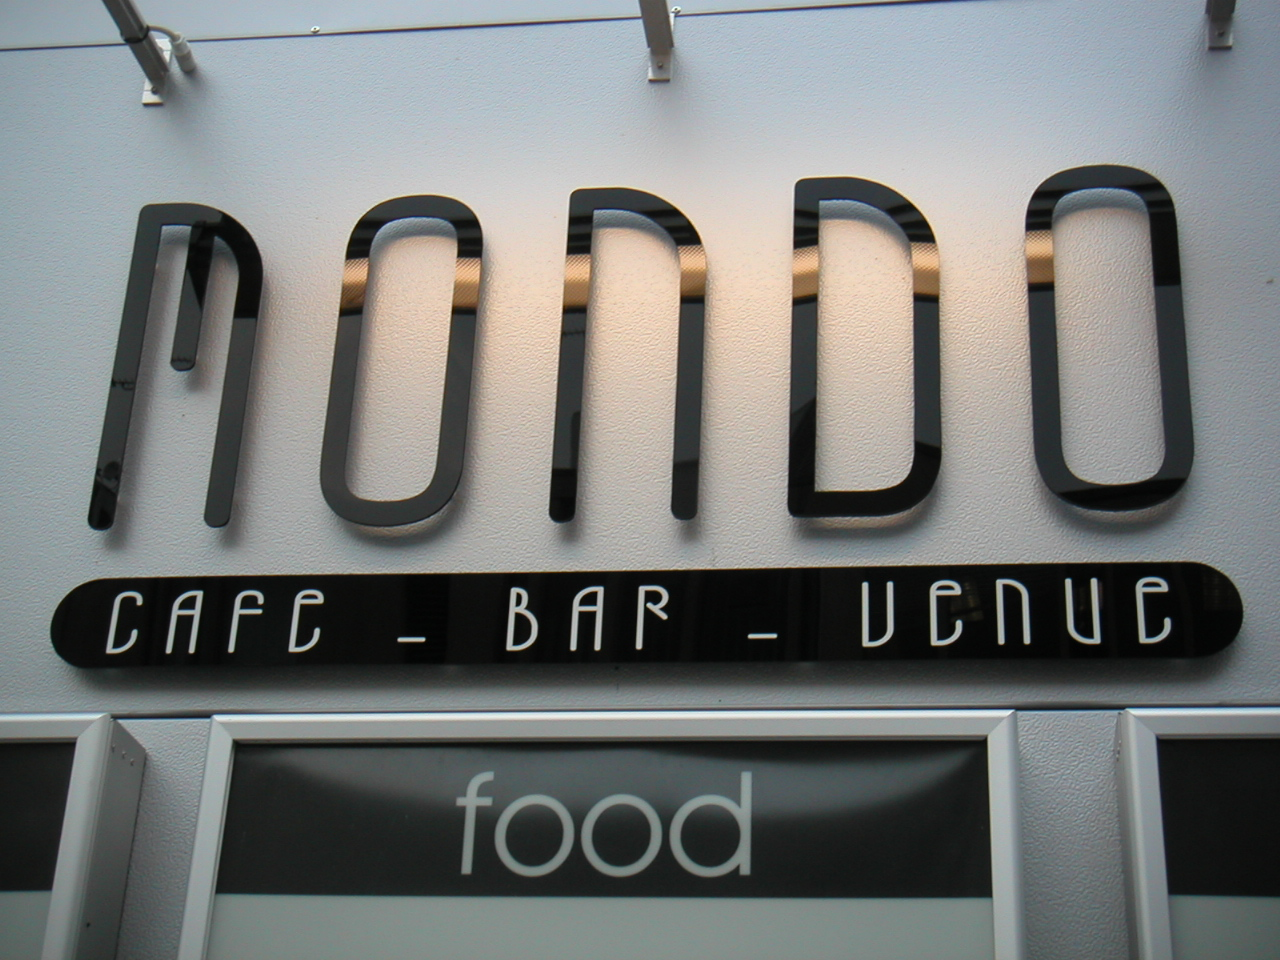
\includegraphics[width=0.75\textwidth]{figs/img_139.jpg}
    \caption{Imagem de uma faixada de comércio, ilustrando um caso de STR. Fonte [\citeonline{ICDAR2013}]}
    \label{fig:str-example}
\end{figure}

% TODO Esse paragrafo parece que ficou misturos niveis de abstrações diferentes. REVISAR
As soluções para problemas de STR, para lidarem com o nível de generalização necessário para reconhecer texto nos mais diversos casos, são largamente 
baseadas nos conceitos de aprendizado profundo, que demonstram conseguir ir um passo à frente no quesito reconhecimento de padrões em comparação às 
técnicas clássicas de processamento de imagem e conseguirem ser aplicadas com eficiência sobre imagens, sendo a aplicação das redes neurais convolucionais, 
comumente abreviadas para CNN pelo nome em inglês \textit{Convolutional Neural Networks}, um divisor de águas na evolução dessas soluções. 
[\citeonline{DetcRecogWild,StrDlEra}].

A pesquisa e experimentação de novos métodos para resolver os mais diferentes problemas que permeiam o STR ainda é atual, com trabalhos 
publicados recentemente.
Em [\citeonline{KPN}], por exemplo, é proposta uma nova arquitetura de detecção, abreviada por KPN pelo nome em inglês \textit{Kernel Proposal Network}), 
utilizando redes convolucionais e segmentação semântica para melhorar a detecção das fronteiras de palavras.

Já em [\citeonline{DEER}], uma solução unificada de localização e reconhecimento é sugerida utilizando redes convolucionais inspirada em soluções de 
detecção de objetos baseadas em codificadores \textit{Transformers} [\citeonline{Transformer}], que, no que lhes concerne, utilizam métodos de atenção. 
As regiões de texto são localizadas apenas por um ponto de referência central, não por uma área bem definidas como é comum. Posteriormente um decodificador 
é utilizado para gerar a sequência de caracteres no entrono do ponto de referência.

\section{Objetivo}

O principal objetivo deste trabalho de graduação é desenvolver e avaliar uma solução integrada de reconhecimento de texto em cenas a parir do uso de 
componentes para detecção e reconhecimento isolados que já fizeram parte do estado da arte, respectivamente CRAFT e CRNN.

Como objetivo complementar, de modo a gerar uma prova de conceito sobre a solução desenvolvida, a partir do uso de provedores de computação em nuvem, 
hospedar uma aplicação \textit{web} para disponibilizar o uso da solução desenvolvida na Internet.

\section{Considerações finais}
Dada a importância do aprendizado profundo, e em especial das CNNs nesse contexto de detecção e reconhecimento de texto, o próximo capítulo irá 
apresentar alguns conceitos básicos associados a essas estruturas.
\chapter{Fundamentação Teórica}

\lipsum[43-45]

\section{Considerações Finais}

\lipsum[23]

\chapter{Metodologia}\label{cap:metodologia}

Uma vez introduzida a temática deste trabalho graduação, seu objetivo e os principais conceitos que o circundam, é possível agora abordar as etapas 
percorridas para executá-lo e, eventualmente, possibilitar que outros, iniciantes no estudo de aplicações de detecção e reconhecimento de texto, 
consigam reproduzi-lo, provendo uma documentação detalhada do caminho tomado durante o desenvolvimento do trabalho.

Sob ótica de todo o ciclo de desenvolvimento deste trabalho de graduação, houveram quatro grandes marcos que servirão para estruturar esse capítulo:

\begin{enumerate}
    \item Experimentação com soluções de reconhecimento e detecção de texto.
    \item Desenvolvimento da solução fim-a-fim a partir de detectores e reconhecedores de texto.
    \item Avaliação da solução fim-a-fim proposta.
    \item Publicação da solução em ambientes de computação em nuvem.
\end{enumerate}

% 1. Experimentação com soluções de reconhecimento e detecção de texto
% 2. Desenvolvimento da solução fim-a-fim a partir de detectores e reconhecedores de texto
% 3. Avaliação da solução fim-a-fim proposta
% 4. Publicação da solução em ambientes de computação em nuvem

Dessa forma, as sub-seções a seguir detalharão cada uma dessas etapas, sob perspectiva da experiência do autor durante a execução deste 
trabalho de graduação.

\section{Experimentação com soluções de reconhecimento e detecção de texto}\label{sec:metodologia_experimentacao}

Apesar de já ter sido mencionado a escolha do componente de detecção, CRAFT, e de reconhecimento, CRNN, não foi abordado o processo adotado 
que culminou nessa escolha. Nessa seção será abordado um pouco da motivação sobre essas escolhas, sob caráter mais técnico e prático sobre 
as soluções disponíveis publicamente, sendo de fácil acesso através da Internet. 

A partir de uma rápida busca na Internet, em especial na plataforma do GitHub\footnote{https://github.com}, hospedeiro de repositórios de 
código-fonte versionados pela ferramenta Git, famoso sistema controlador de versão, é possível encontrar diversos repositórios mencionando 
soluções para detecção e reconhecimento de texto em cenas, às vezes até mesmo repositórios oficiais, oferecidos pelos autores de trabalhos 
famosos na área, como é o próprio exemplo do detector de texto CRAFT.

No entanto, uma grande dificuldade para de fato conseguir executar o código desses repositórios é satisfazer os requisitos e dependências 
minímas, muitas vezes implícitos, por exemplo, a obrigatoriedade de possuir \textit{hardware} com placa gráfica compatível com a versão 
utilizada no momento de desenvolvimento do trabalho original, a indisponibilidade dos modelos pré-treinados para rápida verificação de 
resultados, a base de código incompleta, sem todas as instruções para execução ou com dependências em versões antigas da linguagem de 
programação, bibliotecas e/ou \textit{frameworks}, entre outros.

Outro ponto de grande valor na escolha dos métodos aplicados neste trabalho é a compatibilidade entre os métodos de detecção e reconhecimento. 
Como o grande objetivo deste trabalho se baseia na integração dessas soluções para trabalharem juntas, o caminho mais simples nessa linha é 
que ambos projetos consigam se executados no mesmo ambiente de desenvolvimento, com dependências em bibliotecas e \textit{frameworks} parecidos, 
se não, iguais, para que não houvessem conflitos entre ambos os projetos que trouxessem problemas em tempo de execução.

Na escolha do método de detecção de texto, a partir de uma revisão de trabalhos anteriores da área, foi considerado e, até certo ponto, 
experimentado, códigos oficiais e re-implementações publicas dos seguintes trabalhos:

\begin{itemize}
    \item EAST [\citeonline{EAST}], com implementações dos usuários \textit{argman}\footnote{https://github.com/argman/EAST} e 
    \textit{jandz}\footnote{https://github.com/janzd/EAST}

    \item TextBoxes++ [\citeonline{TxtBoxPlus}], com implementação do usuário \textit{MhLiao}\footnote{https://github.com/MhLiao/TextBoxes\_plusplus}

    \item PixelLink [\citeonline{pixellink}], com implementação do usuário \textit{ZJULearning}\footnote{https://github.com/ZJULearning/pixel\_link}

    \item CRAFT [\citeonline{CRAFT}], com implementação do usuário \textit{clovaai}\footnote{https://github.com/clovaai/CRAFT-pytorch}
\end{itemize}

Por fim, o que foi mais acessível em relação aos pontos citados anteriormente foi o código-fonte do CRAFT. Os autores desenvolveram o modelo em 
Python, usando o framework PyTorch\footnote{https://pytorch.org}, biblioteca popular na comunidade, facilitando na escolha de projetos para 
integrar o reconhecimento de texto. Os autores também disponibilizaram os modelos pré-treinados para detecção de texto em cenas, o que é um 
grande diferencial, já que os procedimentos de treinamento dessas soluções não são triviais, além de costumarem ser custosos temporal 
e computacionalmente, o que desviaria o foco do objetivo desse trabalho. Adicionalmente, o código-fonte contém instruções minímas de como executar 
o modelo pré-treinado, que se mostraram suficientes para iniciantes sem muita experiencia prévia com a linguagem de programação e em trabalhos 
de detecção de texto. Outro diferencial foi a possibilidade de executar o modelo pré-treinado em equipamento físico sem aceleração gráfica, mesmo 
que com a penalização no tempo de execução. Essa capacidade foi de grande valor, já que os componentes compatíveis não são baratos, dado o contexto 
atual de cripto-moedas e escassez de processadores gráficos no mercado.

Agora sobre a escolha do método de reconhecimento, como o detector escolhido usa a linguagem Python e o framework PyTorch, a lista de métodos 
disponíveis foi filtrada por esses critérios. Uma implementação do CRNN em PyTorch foi escolhida, pois, atendia os critérios de compatibilidade 
com a linguagem, framework e bibliotecas que o CRAFT depende, aliado ao fato do CRNN ser uma solução popular, com implementação sucinta e, 
novamente, de fácil execução a partir de um modelo pré-treinado, o que também foi fornecido pelo autor da implementação.

Durante todo o processo de experimentação e de desenvolvimento, a plataforma Paperspace\footnote{https://www.paperspace.com} foi de grande valor. 
A Paperspace é uma empresa provedora de computação em nuvem especializada em infraestrutura para aplicações de aprendizado de máquina, disponibilizando 
gratuitamente ambientes de Jupyter Notebooks em máquinas com aceleração gráfica gratuitamente para fins de estudo e experimentação, com características 
similares ao Google Colab\footnote{https://colab.research.google.com/}.

Executar o CRAFT e o CRNN a partir dos respectivos repositórios originais não demandaram muitas configurações ou customizações específicas além da 
configuração correta do ambiente de desenvolvimento facilitado a ferramenta Conda, que será introduzida com mais detalhes na Seção \ref{sec:metodologia_desenvolvimento}.
 Ambos repositórios já continham \textit{scripts} básicos para testar a predição a partir dos modelos pré-treinados, então, tanto para o CRAFT, 
 quanto o CRNN, executar os modelos com imagens de testes já incluídas nos repositórios originais ou com outras imagens quaisquer demandava ajustes 
 mínimos para ajustar as referências para leitura da imagem de entrada e re-executar os \textit{scripts} de predição.

Sobre as características das entradas e saídas dos modelos escolhidos, durante a detecção através do modelo CRAFT não existem restrições notáveis a 
respeito dos dados de entrada. São esperadas imagens, que podem conter tamanhos variados, e, contando que possam ser abertas pelo \textit{script} de 
detecção, são passíveis de serem processadas pelo modelo. Como citado na Seção \ref{craft}, a rede de detecção produz imagens que descrevem a localização 
de cada região de caractere e o nível de afinidade das vizinhanças dos caracteres detectados. O processamento dessas imagens brutas que a rede produz é 
disponibilizado pelos autores e faz parte do repositório original, portanto o código que consegue derivar as coordenadas de \textit{bounding-boxes} 
para cada palavra já é disponibilizado pelos autores do CRAFT. A Figura \ref{fig:methodology_craft_example} exemplifica os resultados de detecção originais 
do CRAFT e demonstram a capacidade de produzir tanto os arquivos brutos, que ilustram os resultados da rede de detecção, quanto uma visualização sobre a 
imagem de entrada, desenhando os contornos retangulares em volta das palavras detectadas.

\begin{figure}
    \centering
    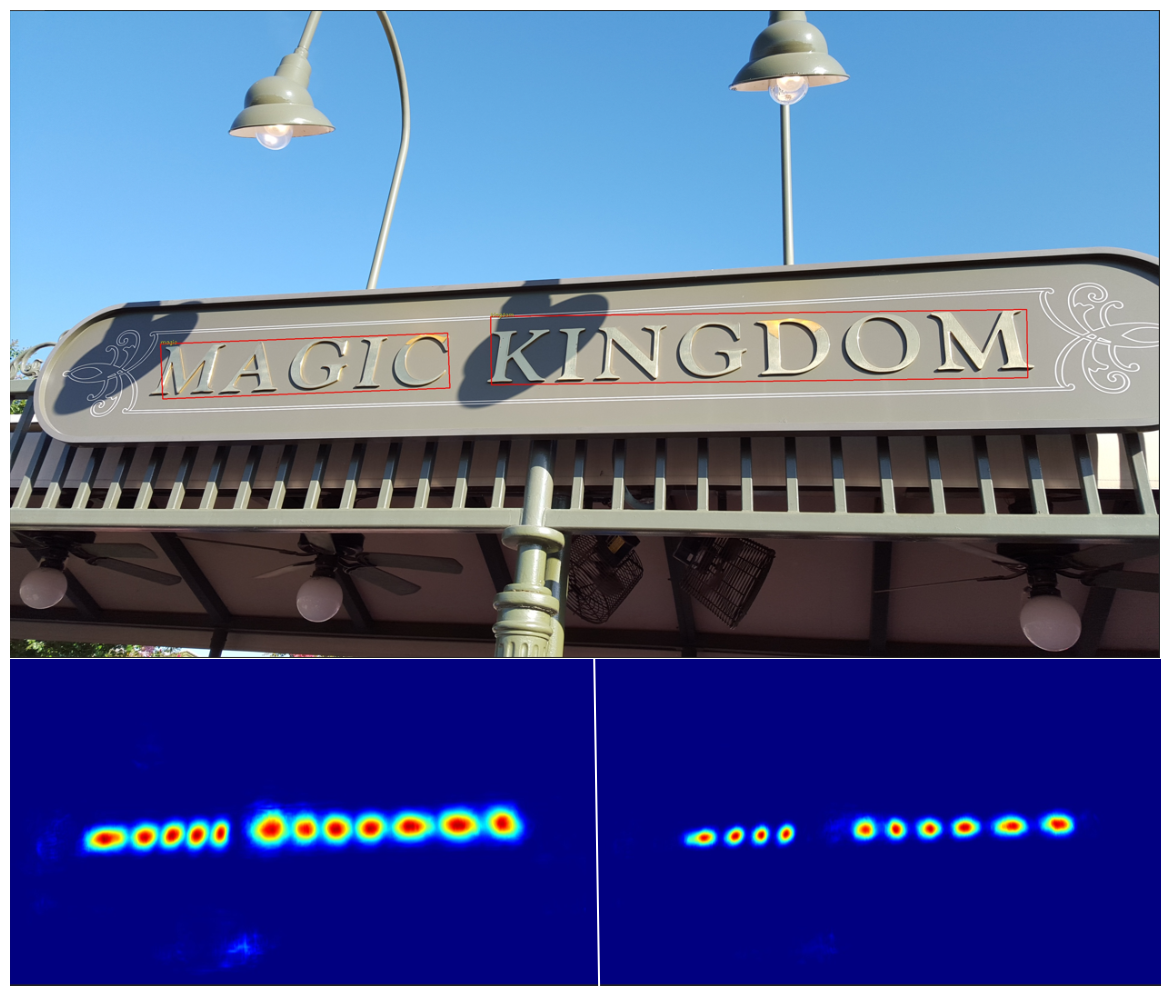
\includegraphics[width=0.8\textwidth]{figs/craft-exmaple.png}
    \caption{Exemplo das imagens geradas a partir da detecção pelo CRAFT sobre uma imagem autoral.}
    \label{fig:methodology_craft_example}
\end{figure}

Agora sobre o modelo de reconhecimento, para as imagens de entrada, espera-se que contenham apenas uma palavra por imagem e devem respeitar limites de 
dimensão impostas pela rede que, na implementação utilizada, já são aplicadas durante a execução do \textit{script} de predição, limitando a altura das 
imagens em 32 píxeis. O resultado da predição é a impressão do texto reconhecido ao final da execução do programa. 

A próxima sub-seção abordará, com um pouco mais de detalhes, como as duas soluções escolhidas foram integradas em uma mesma base de código e como os 
resultados do CRAFT foram processados para poderem alimentar a implementação do CRNN, completando a solução fim-a-fim do reconhecimento de texto. 

\section{Desenvolvimento da solução fim-a-fim a partir de detectores e reconhecedores de texto}\label{sec:metodologia_desenvolvimento}

De modo a aplicar o reconhecimento, utilizando o CRNN, exatamente sobre o texto detectado e localizado pelo CRAFT, escolheu-se utilizar o repositório com 
o código-fonte do detector CRAFT como base inicial para a aplicação de reconhecimento fim-a-fim e, a partir dele, adicionar a solução de reconhecimento 
dentro da mesma base de código e fazer com que ambas tenham todas as dependências necessárias para conseguirem executar seu processamento. Em outras palavras, 
foi necessário preparar um ambiente de desenvolvimento Python com todas a dependências, ao nível de linguagem de programação, bibliotecas e 
\textit{frameworks}, instalados e sem conflitos, com tanto as bibliotecas que são dependências obrigatórias para a implementação do CRAFT quanto as 
bibliotecas utilizadas na implementação do CRNN.

Para a gestão de ambientes de desenvolvimento e suas dependências, foi utilizado uma ferramenta no ecossistema Python chamada Conda, mantida pela empresa 
Anaconda. Com essa ferramenta é possível criar ambientes virtuais Python e instalar todas as dependências necessárias dentro desses ambientes virtuais 
usando poucas instruções na linha de comando do computador. A própria ferramenta fornece meios para de gerir os ambientes virtuais criados e otimiza a 
instalação de pacotes dentro desses ambientes de forma que conflitos sejam evitados, resolvendo as versões dos pacotes instalados de forma que sejam 
compatíveis entre si e compatíveis com a versão da linguagem Python escolhida para o ambiente. Uma grande vantagem de usar esse gerenciador de ambientes 
Python é a possibilidade de reproduzir qualquer ambiente virtual previamente configurado a partir de um arquivo de configuração, do tipo YAML, que lista 
todos os pacotes instalados em um ambiente virtual para que, a partir desse arquivo, a ferramenta consiga remontar o mesmo ambiente sem precisar de 
configurações manuais novamente.

Entrando mais no caminho percorrido para integrar as duas soluções, a primeira etapa foi replicar os repositórios para a conta pessoal do autor no GitHub. 
Esse processo na plataforma Github se chama \textit{fork} e, em geral, é utilizado para possibilitar que outras pessoas consigam desenvolver coisas 
novas a partir da base de código original sem ter o risco de empurrar mudanças no repositório original inadvertidamente. Dessa forma, ambos os repositórios 
foram replicados para a conta pessoal do autor e todo o desenvolvimento deste trabalho foi feito nos repositórios replicados.

A partir dos repositórios replicados, foi utilizado um recurso da ferramenta de versionamento, o Git, que possibilita a composição de repositórios de modo 
a facilitar a sincronização das bases de códigos. O recurso em questão é a criação de sub-módulos em um repositório Git. Usando o comando abaixo a partir 
do repositório replicado do detector, foi gerado um relacionamento entre as duas bases de código, sendo que o repositório do CRNN agora é visto como um 
sub-módulo do repositório do CRAFT, e, a partir disso, é possível baixar, usar, evoluir a base de código do repositório do CRNN diretamente do repositório 
do CRAFT. Isso fez com que ambas soluções já tenham visibilidade uma da outra, mas ainda não fez com que trabalhem juntas.

\begin{minted}{bash}
    git submodule add https://github.com/mmilani1/crnn.pytorch
\end{minted}

Com as soluções na mesma base de código, uma etapa importante é a garantir que ambas ainda funcionam isoladamente e se validar a compatibilidade das dependências 
de cada uma. Como mencionado na Seção \ref{sec:metodologia_experimentacao}, uma das motivações da escolha especificamente dessas duas implementações citadas foi 
justamente a maior proximidade em \textit{frameworks} e bibliotecas que utilizam, inclusive a possibilidade de ambas soluções poderem ser executadas sem a 
necessidade de aceleração gráfica. Dessa forma não houve problemas em executar separadamente cada solução, mesmo compartilhando o mesmo ambiente virtual. 
O arquivo YAML com a descrição do ambiente virtual pode ser consultado diretamente do repositório com a implementação ou no Apêndice \ref{apd:yaml-desenvolvimento}.

A partir deste ponto já se torna possível trabalhar com os modelos de detecção e reconhecimento para integrá-los, de alguma forma. O objetivo ao fim da integração 
é conseguir reconhecer texto em imagens de cena, para isso, a ideia é evoluir a extração de resultados do modelo de detecção CRAFT para gerar uma lista de 
recortes das regiões de texto da imagem original e implementar um algoritmo que execute o modelo de reconhecimento CRNN para cada um desses recortes.

Conforme detalhado na Seção \ref{sec:metodologia_experimentacao}, a implementação do CRAFT fornecida é didática o suficiente com os resultados da detecção, 
gerando visualizações dos resultados através de arquivos de texto contendo as coordenadas das regiões de texto detectadas. Isso demonstra que, em algum ponto 
do código original as coordenadas dessas regiões de texto foram manuseadas pelos autores do modelo e, consequentemente, poderão ser manuseadas no 
desenvolvimento da solução integrada de modo a gerar os recortes que serão posteriormente consumidos pelo modelo reconhecimento. O Algoritmo \ref{alg:pseudo_codigo} 
apresenta o pseudo-algoritmo com as etapas do processamento executado.


\begin{algorithm}
\caption{Pseudo-Código da integração entre a detecção e o reconhecimento de texto}\label{alg:pseudo_codigo}
\begin{algorithmic}
\State $imagem \gets{lerEntrada()}$
\State $palavras \gets{[ ]}$
\State $regioesDeTexto \gets{executaDeteccaoCRAFT(imagem)}$
\For{$regiaoDeTexto \in regioesDeTexto$}
    \State $recorte \gets{recortarTextoDaImagemOriginal(imagem,regiaoDeTexto)}$
    \State $palavra \gets{executaReconhecimentoCRNN(recorte)}$
    \State $palavras \gets{paralvras + [palavra]}$
\EndFor
\State{}
\Return{$palavras$}
\end{algorithmic}
\end{algorithm}

% ```
% imagem = lerEntrada()
% vetoreDePalavrasReconhecidas = []
% vetorDeRegioesDeTexto = detectorCRAFT(imagem)

% para cada regiao em vetorDeRegioesDeTexto:
%   regiaoDeTextoExtraida = extrairRegiaoDaImagemOriginal(regiao)
%   palavra = reconhecimentoCRNN(regiãoDeTextoExtraida)
%   vetorDePalavrasReconhecidas << palavra

% retorna vetorDePalavrasReconhecidas
% ```

Para efetuar o recorte das regiões de texto localizadas e fornecidas na saída do modelo de detecção, foi utilizado um par de funções da biblioteca 
OpenCV, especializada em ferramentas voltadas para visão computacional. As funções utilizadas foram \texttt{cv2.getPerspectiveTransform} e 
\texttt{cv2.warpPerspective}.
A primeira função é responsável por gerar uma matriz de transformação de áreas quadrangulares e recebe duas sequencias de pontos. A primeira 
sequência contém os vértices da área quadrangular a ser transformada, no caso desse trabalho, são as coordenadas da \textit{bounding-box} de uma 
palavra detectada. Já a segunda sequência de pontos representa os vértices da imagem de saída, para onde o cada um dos pontos da primeira 
sequência serão transportados após a aplicação da transformação.
A segunda função é responsável por aplicar a matriz de transformação, gerada a partir da execução do comando \texttt{cv2.getPerspectiveTransform}, 
sobre a imagem onde o texto foi detectado. Dessa forma conseguimos recortar as palavras detectadas da imagem original de forma cada é possível 
posteriormente passar as referências desses recortes para o modelo de reconhecimento diretamente, já que os dados de entrada esperados pelo CRNN 
são imagens que contém idealmente uma palavra para reconhecimento. A Figura \ref{fig:methodology_pipeline} ilustra, em alto nível, as etapas do 
processamento que compõem as soluções de STR fim-a-fim deste trabalho.

\begin{figure}
    \centering
    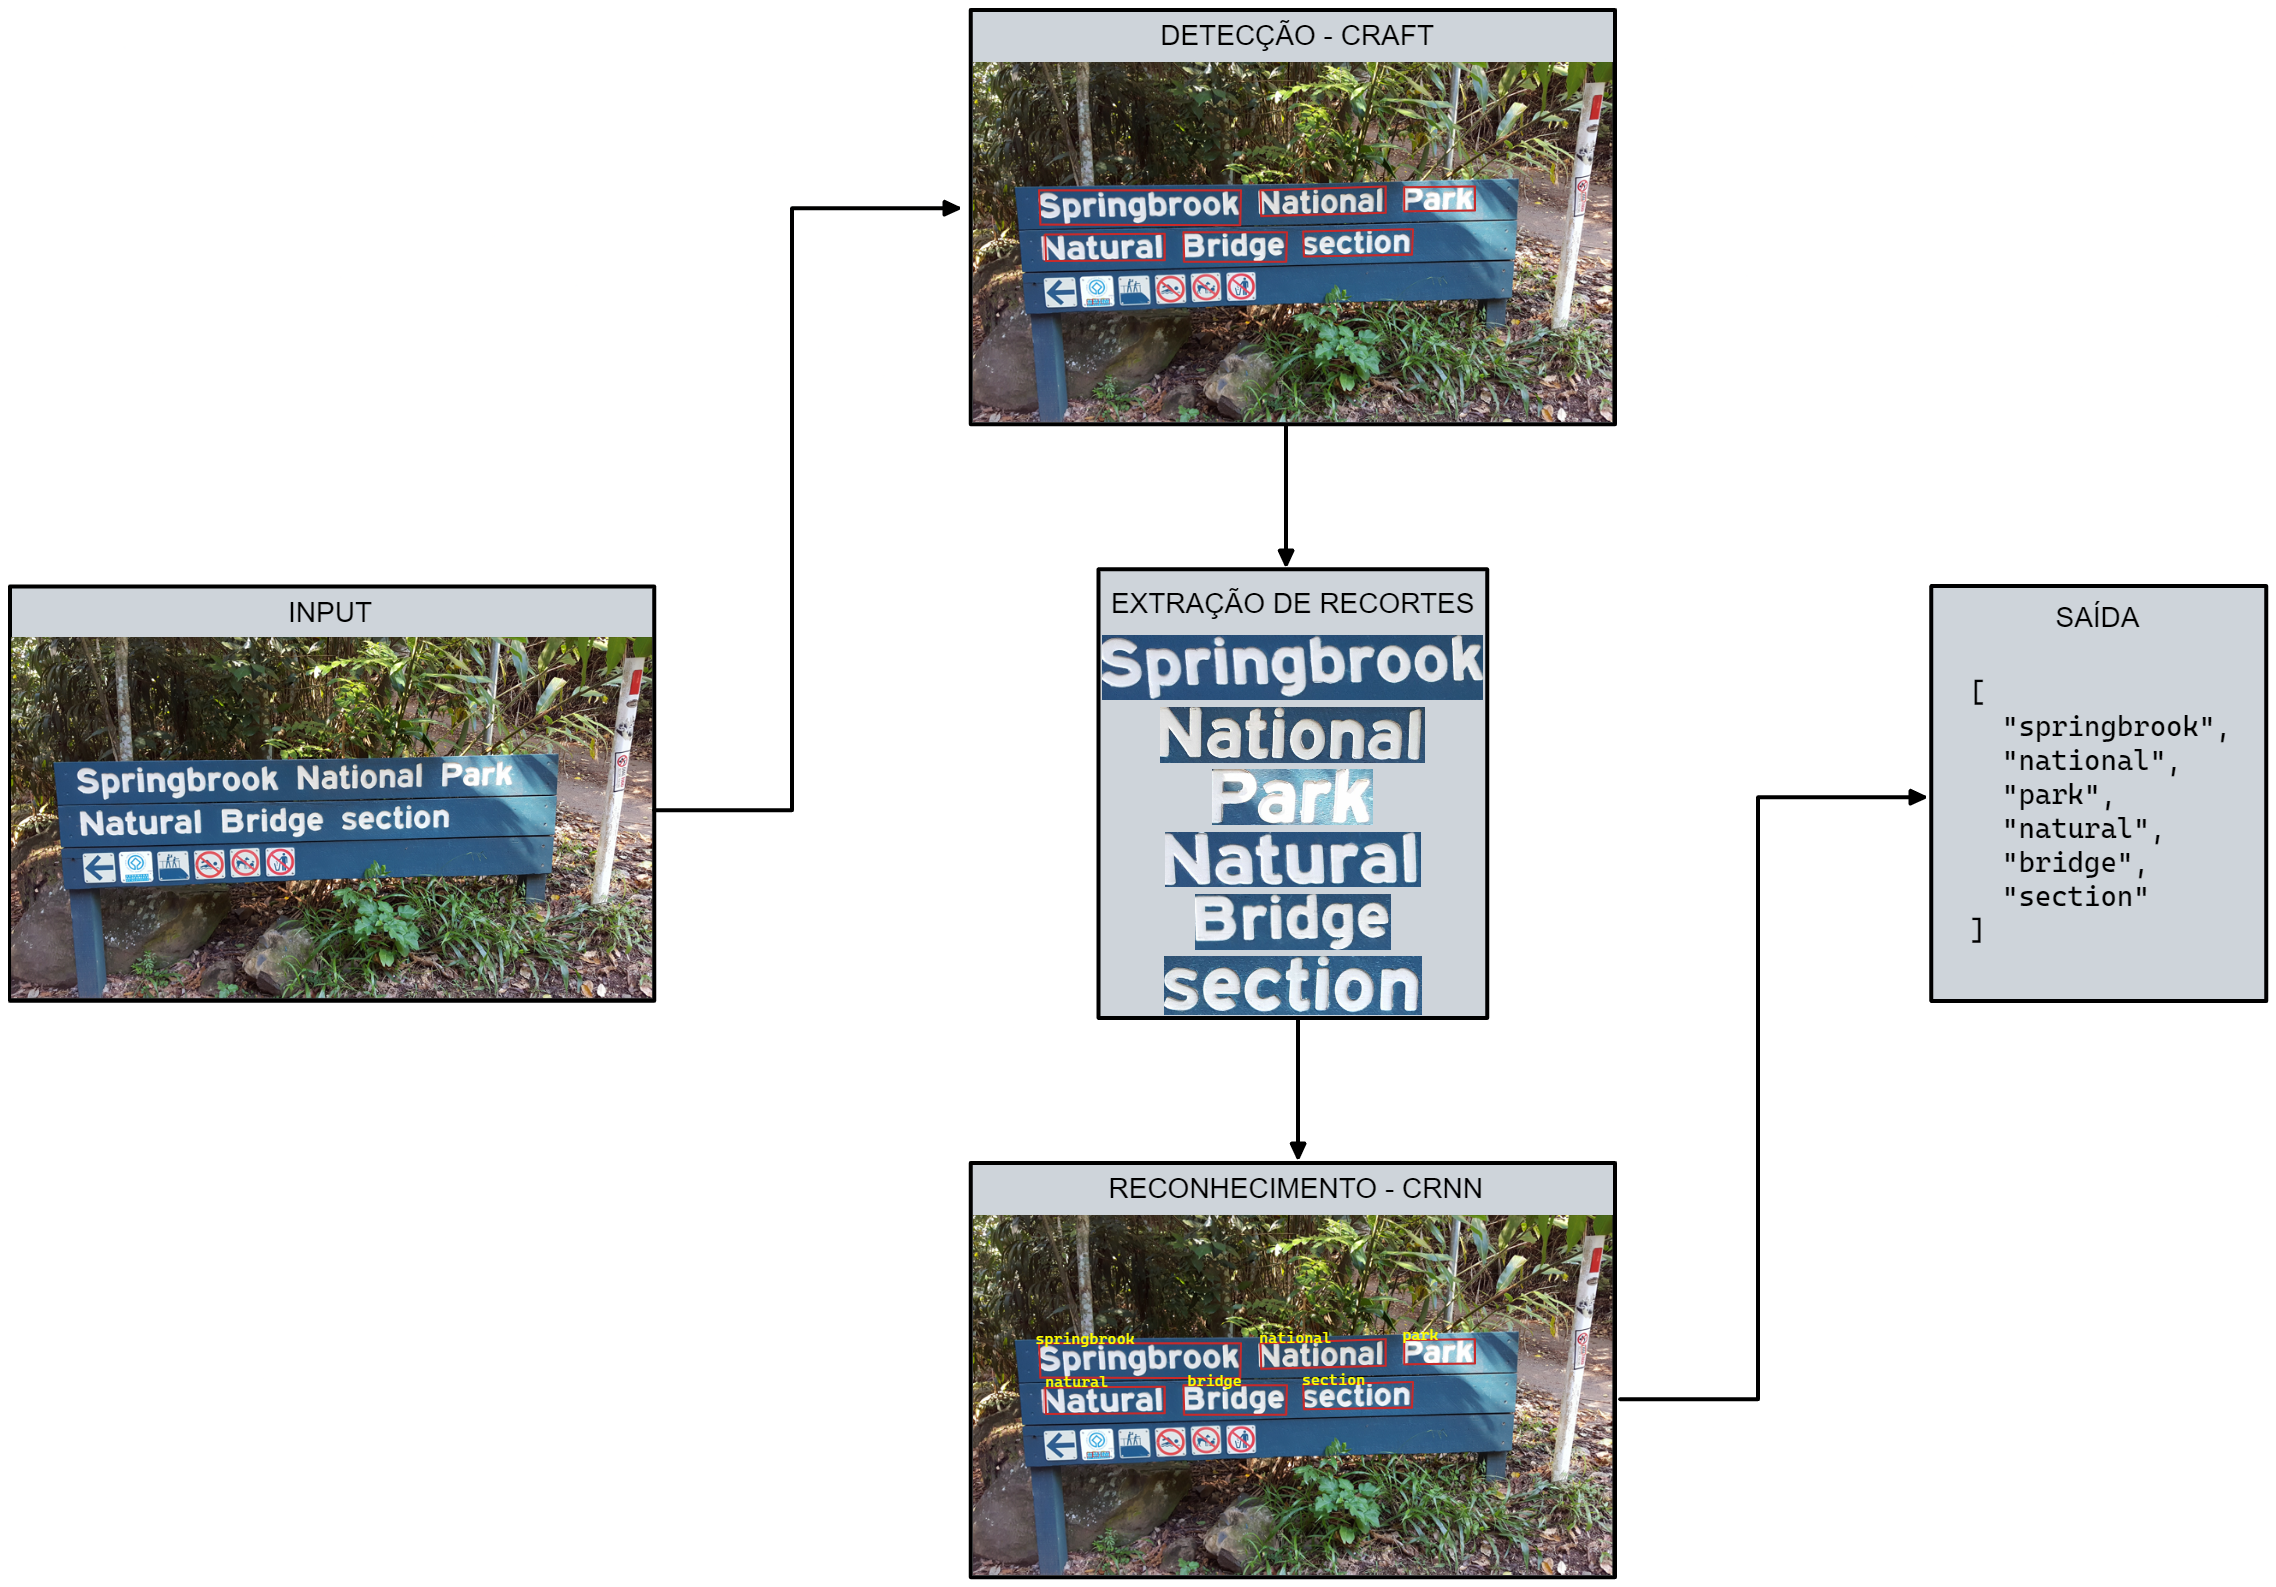
\includegraphics[width=\textwidth]{figs/metodologia-pipeline.png}
    \caption{Ilustração das etapas de processamento da solução proposta.}
    \label{fig:methodology_pipeline}
\end{figure}

Ao fim dessas alterações, integrando os dois modelos de detecção e reconhecimento, já temos uma solução simples de reconhecimento de texto em cenas 
que pode ser classificada como \textit{end-to-end}, que contempla tanto a detecção quanto o reconhecimento dentro de uma mesma aplicação. A próxima 
etapa é conseguir avaliar a eficácia desse novo desenvolvimento. A próxima seção introduzirá os métodos e métricas utilizadas para avaliar a solução.

\section{Método de avaliação da solução proposta}\label{sec:methodology_validation}

A avaliação analítica da solução proposta neste trabalho é baseada na forma de avaliação da plataforma \textit{Robust Reading Competition}\footnote{https://rrc.cvc.uab.es/}, 
disponibilizado pelo Centro de Visão Computacional da Universidade Autônoma de Barcelona. Essa plataforma organiza competições em torno de 
problemas reais de visão computacional e tipicamente essas competições se relacionam com a Conferência Internacional sobre Análise e Reconhecimento 
de Documentos, abreviada como ICDAR a partir do nome da conferência em inglês. Diversas bases de dados que são amplamente adotados para 
treino e avaliação de modelos de reconhecimento de texto levam no nome a menção ao ICDAR, por introduzirem a base de dados e os desafios 
propostos, fomentando novos trabalhos na área.

Essa seção irá introduzir as bases de dados utilizadas para avaliação, as métricas utilizadas e o processo de avaliação da solução apresentada 
utilizando as ferramentas de avaliação disponibilizadas pela plataforma RRC.

\subsection{Base de Dados}\label{sec:methodology_datasets}

Conforme mencionado anteriormente, as bases de dados dos desafios vinculados ao ICDAR são muito utilizados por trabalhos voltados à detecção e 
reconhecimento de texto. Ambos os modelos utilizados no desenvolvimento deste trabalho referem-se às bases de dados ICDAR: O CRAFT cita as bases 
de dados ICDAR 2013 [\citeonline{ICDAR2013}], ICDAR 2015 [\citeonline{ICDAR2015}] e ICDAR 2017 [\citeonline{ICDAR2017}] como bases de treinamento 
e de validação em quanto o CRNN se refere ao ICDAR 2003 [\citeonline{ICDAR2003}] e ICDAR 2013 como bases de imagens para validação. As bases de 
dados utilizadas para a avaliação deste trabalho foram o ICDAR 2011 [\citeonline{ICDAR2011}], base para o primeiro desafio da plataforma RRC 
chamado \textit{Reading Text in Born-Digital Images}, e o ICDAR 2013, sendo a base para o segundo desafio da plataforma RRC, chamado \textit{Focused Scene Text}.

\subsubsection{ICDAR 2011}\label{sec:datasets_icdar2011}
O ICDAR 2011 [\citeonline{ICDAR2011}] conta com 410 imagens para treino e 141 imagens para validação no contexto de anúncios de Internet e anexos 
de \textit{e-mails}, com palavras em geral na horizontal e anotadas com \textit{bounding-boxes} retangulares ao nível de palavras. As imagens 
são anotadas com a localização de cada palavra com coordenadas das \textit{bounding-boxes} retangulares, que servem como gabarito para soluções 
de detecção e localização. Cada imagem também conta com a transição das palavras para servir como gabarito de soluções de reconhecimento. 
A Figura \ref{fig:icdar2011_examples} expõe algumas imagens desta base de dados.

\begin{figure}
    \centering
    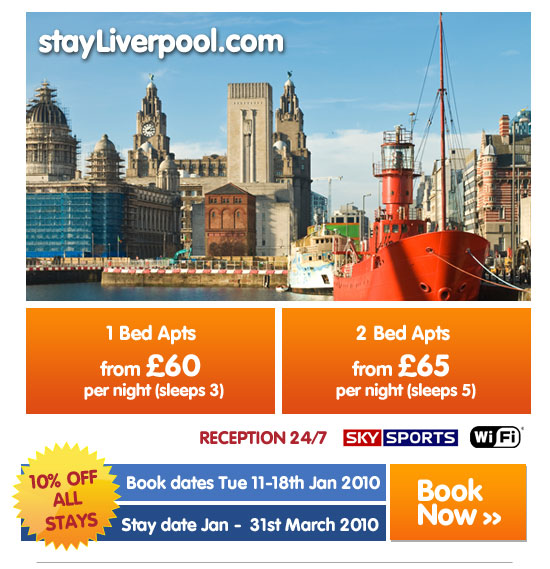
\includegraphics[width=0.3\textwidth]{figs/img_33.png}
    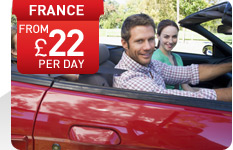
\includegraphics[width=0.3\textwidth]{figs/img_62.jpg}
    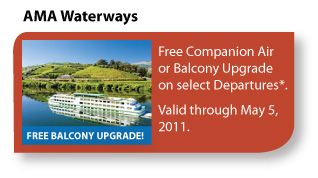
\includegraphics[width=0.3\textwidth]{figs/img_13.jpg}
    \caption{Exemplos de imagens da base de dados ICDAR 2011. Fonte [\citeonline{ICDAR2011}]}
        \label{fig:icdar2011_examples}
\end{figure}

\subsubsection{ICDAR 2013}\label{sec:datasets_icdar2013}
O ICDAR 2013 [\citeonline{ICDAR2013}] conta com 219 imagens para treino e 233 imagens para validação. São imagens de cenas onde, em geral, o texto 
tem boa qualidade e está em destaque, na orientação horizontal. As anotações de gabarito são retangulares ao nível de palavras e contam com a 
transição das mesmas, similarmente às imagens do ICDAR 2011. A Figura \ref{fig:icdar2013_examples} expõe algumas imagens desta base de dados.

\begin{figure}
    \centering
    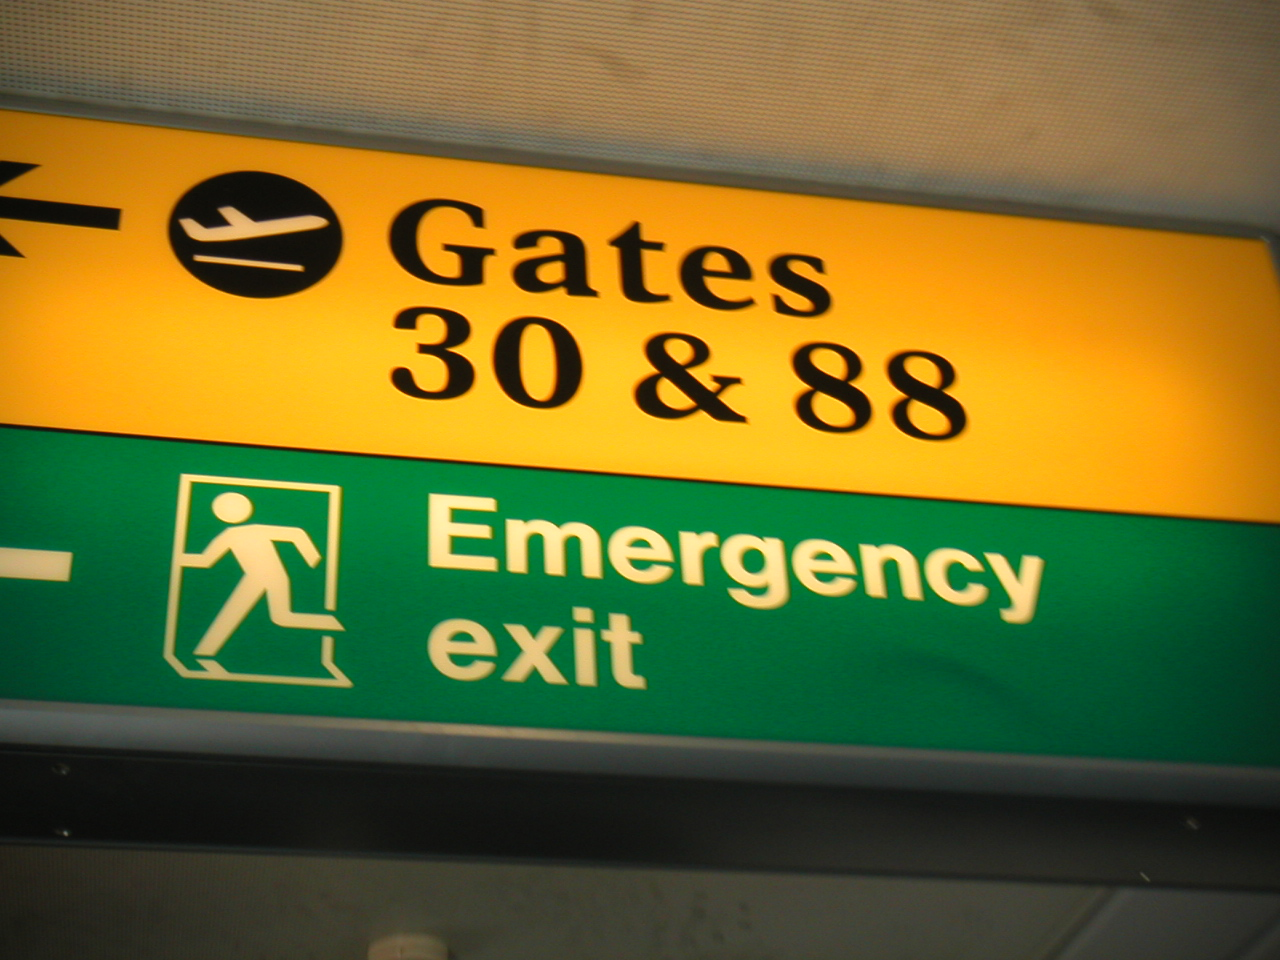
\includegraphics[width=0.3\textwidth]{figs/img_20.jpg}
    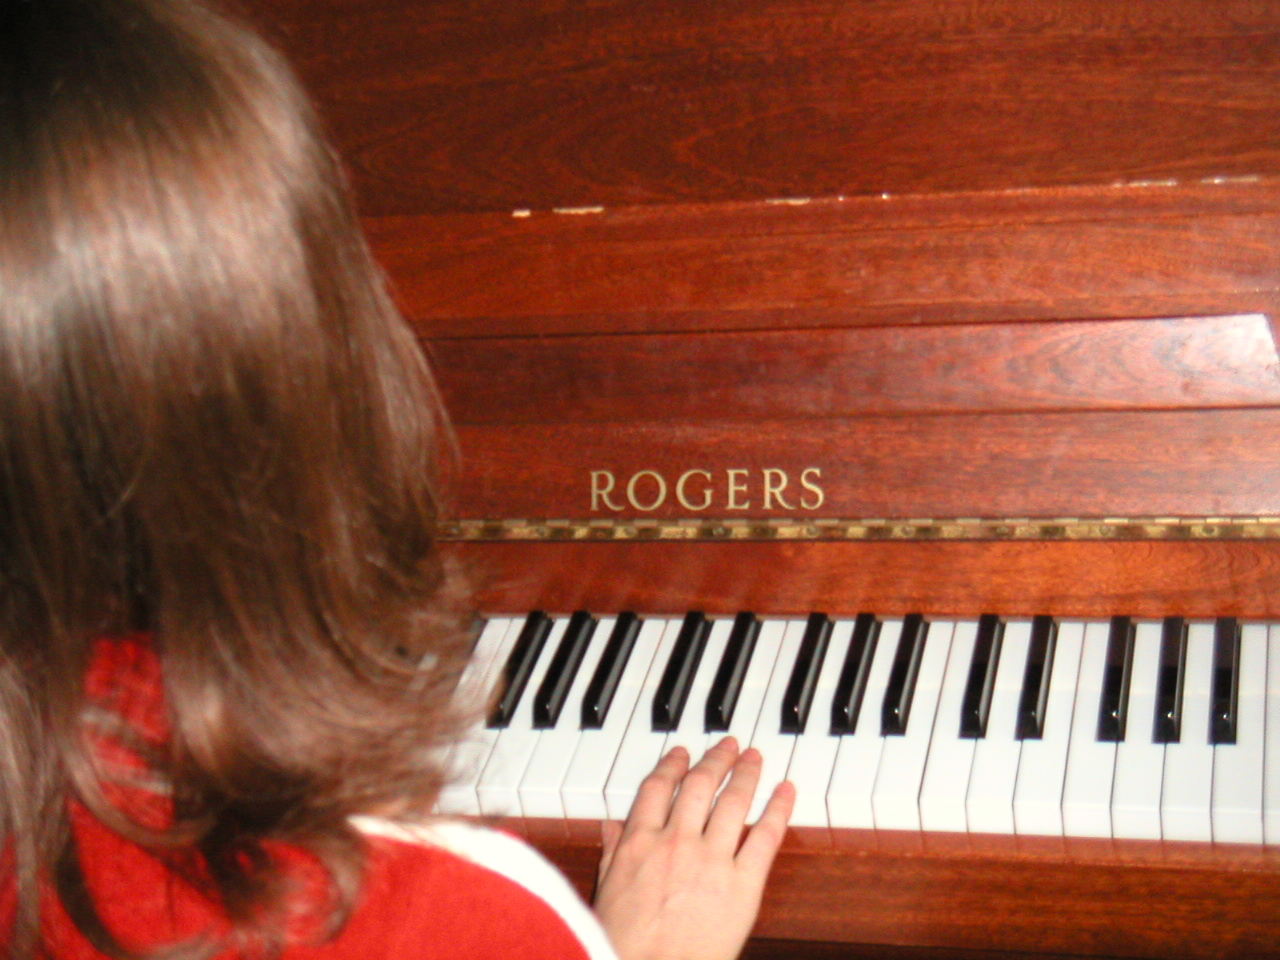
\includegraphics[width=0.3\textwidth]{figs/img_85.jpg}
    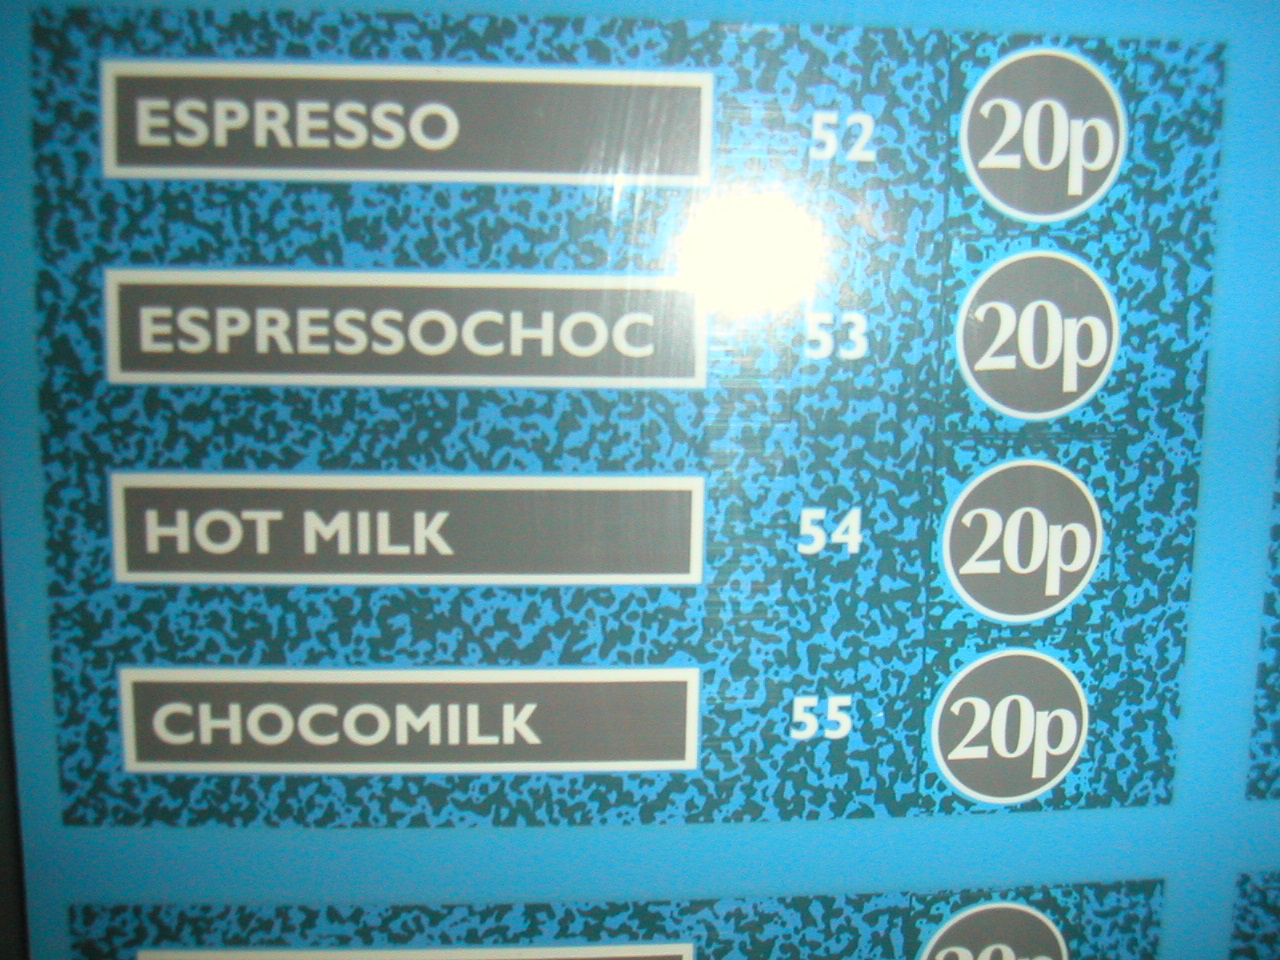
\includegraphics[width=0.3\textwidth]{figs/img_225.jpg}
    \caption{Exemplos de imagens da base de dados ICDAR 2013. Fonte [\citeonline{ICDAR2013}]}
    \label{fig:icdar2013_examples}
\end{figure}

\subsection{Métricas}\label{sec:methodology_metrics}
Em conjunto às bases de dados, são fornecidas meios de avaliação para que cada nova solução que surgir possam ser avaliadas sob os mesmos termos, 
usando os mesmos conceitos e as mesmas métricas. Na plataforma RCC e nas bases de dados que eles disponibilizam são utilizados: precisão, 
\textit{recall} e \textit{F1-Score} (ou H-Mean). A Precisão é a relação dos acertos (verdadeiros positivos) sobre a contagem total de predições 
positivas (verdadeiros positivos e falsos negativos), ou seja, dentre as predições da solução, qual é a porcentagem de acerto. O \textit{Recall} 
relaciona a quantidade de acertos com a quantidade total de casos verdadeiros. O \textit{F1-Score} é basicamente a média harmônica das métricas 
precisão e \textit{recall}.

\begin{equation}
    Precisão = \frac{VP}{VP + FP}
\end{equation}
\begin{equation}
    Recall = \frac{VP}{VP + FN}
\end{equation}
\begin{equation}
    F1Score = 2 \times \frac{Precisão \times Recall}{Precisão + Recall}
\end{equation}

Para determinar se uma predição foi correta existem duas condições: A região de texto detectada deve satisfazer uma métrica característica de 
eficácia em detecção e localização das palavras na imagem chamada IoU, abreviação para \textit{Intersection over Union}, além da transcrição 
predita ser exatamente igual ao gabarito. Para uma predição ser considerada correta, o valor de IoU, que se resume à precisão da detecção, deve 
ser maior ou igual a 50\%.

A métrica de IoU pode ser calculada a partir das coordenadas verdadeiras de uma região de texto, documentadas nas anotações das bases de dados, 
e das coordenadas preditas pelo modelo de detecção. Ambos conjuntos de coordenadas descrevem uma área retangular, para as duas bases de dados 
utilizadas. Com esses dois conjuntos de valores, pode-se avaliar tanto o tamanho da intersecção entre a área predita e a área esperada, quanto o 
tamanho da união entre ambas as áreas. O valor numérico da métrica IoU decorre, conforme sugerido pelo nome da métrica, da divisão entre o 
tamanho da intersecção sobre o tamanho da união entre as áreas preditas e as áreas esperadas.

\subsection{Interface de Validação}\label{sec:methodology_validation_interface}
Na plataforma do RRC é possível avaliar uma solução formalizando a submissão dos resultados diretamente no site da competição, dessa forma os 
resultados ficam registrados na plataforma e pode ser até ranqueada junto a outros trabalhos submetidos. Para cada desafio da plataforma existe 
o ranque de soluções, onde é pode-se observar resultados de outros trabalhos de maneira simples e, quando disponível, até consultar quem são os 
autores, se existe algum repositório público para a base de código, visualizar o artigo do trabalho, etc.

No entanto, submeter os resultados diretamente na plataforma para avaliação remota não é a única opção. É possível também efetuar o \textit{download} 
dos \textit{scripts} que calculam os resultados, nos mesmos moldes da avaliação remota, de modo a executar todo o processo localmente. Essa 
foi a alternativa de avaliação adotada para esse trabalho de graduação.

Para ambos os meios de validação, é necessário preparar arquivos de resultados, para cada imagem da base de dados de validação, com os dados 
necessários para a avaliação. Tanto o ICDAR 2011 quanto o ICDAR 2013 demandam arquivos com o mesmo formato, que se assemelham justamente aos 
arquivos de gabarito dessas bases, e seguem o seguinte formato descrito abaixo. Um exemplo de arquivo de resultado foi disponibilizado no 
Apêndice \ref{apd:exe_resultado}

\begin{itemize}
    \item É necessário gerar um arquivo de texto, para cada imagem, nomeados respeitando o seguinte formato: \texttt{res\_img\_\#.txt}, onde o \texttt{\#} 
    corresponde ao identificador numérico da imagem na base de dados.

    \item Cada arquivo deve ter uma linha para cada palavra detectada e reconhecida.

    \item Cada linha deve conter os seguintes valores, separados por vírgula simples, exatamente na ordem especificada: posição do vértice esquerdo 
    superior da \textit{bounding-box}, vértice direto inferior da \textit{bounding-box} e texto da transição.
\end{itemize}

Após gerar todos os arquivos necessários, resta agregá-los em um arquivo comprimido do tipo ZIP e executar a ferramenta de validação localmente. 
Os arquivos de execução local são escritos em Python e dependem de poucas bibliotecas. Executam um pequeno servidor \textit{web} para servir a aplicação 
de validação. Durante a execução da validação deste trabalho, foi utilizado novamente a ferramenta Conda para gerir essas dependências. O Apêndice 
\ref{apd:yaml-validacao} contém o arquivo que descreve o ambiente virtual utilizado. A Figura \ref{fig:methodology_validation_interface} mostra um 
pouco da interface de usuário que a aplicação fornece, com as funcionalidades de submeter o arquivo comprimido de solução e a Figura 
\ref{fig:methodology_validation_interface_details} mostra a funcionalidade de verificação dos resultados sobre cada imagem, possibilitando a 
análise sobre onde as soluções funcionaram bem e onde não funcionaram tão bem, o que foi feito no contexto da solução proposta nesse trabalho 
no Capítulo \ref{cap:resultados}.

\begin{figure}
    \centering
    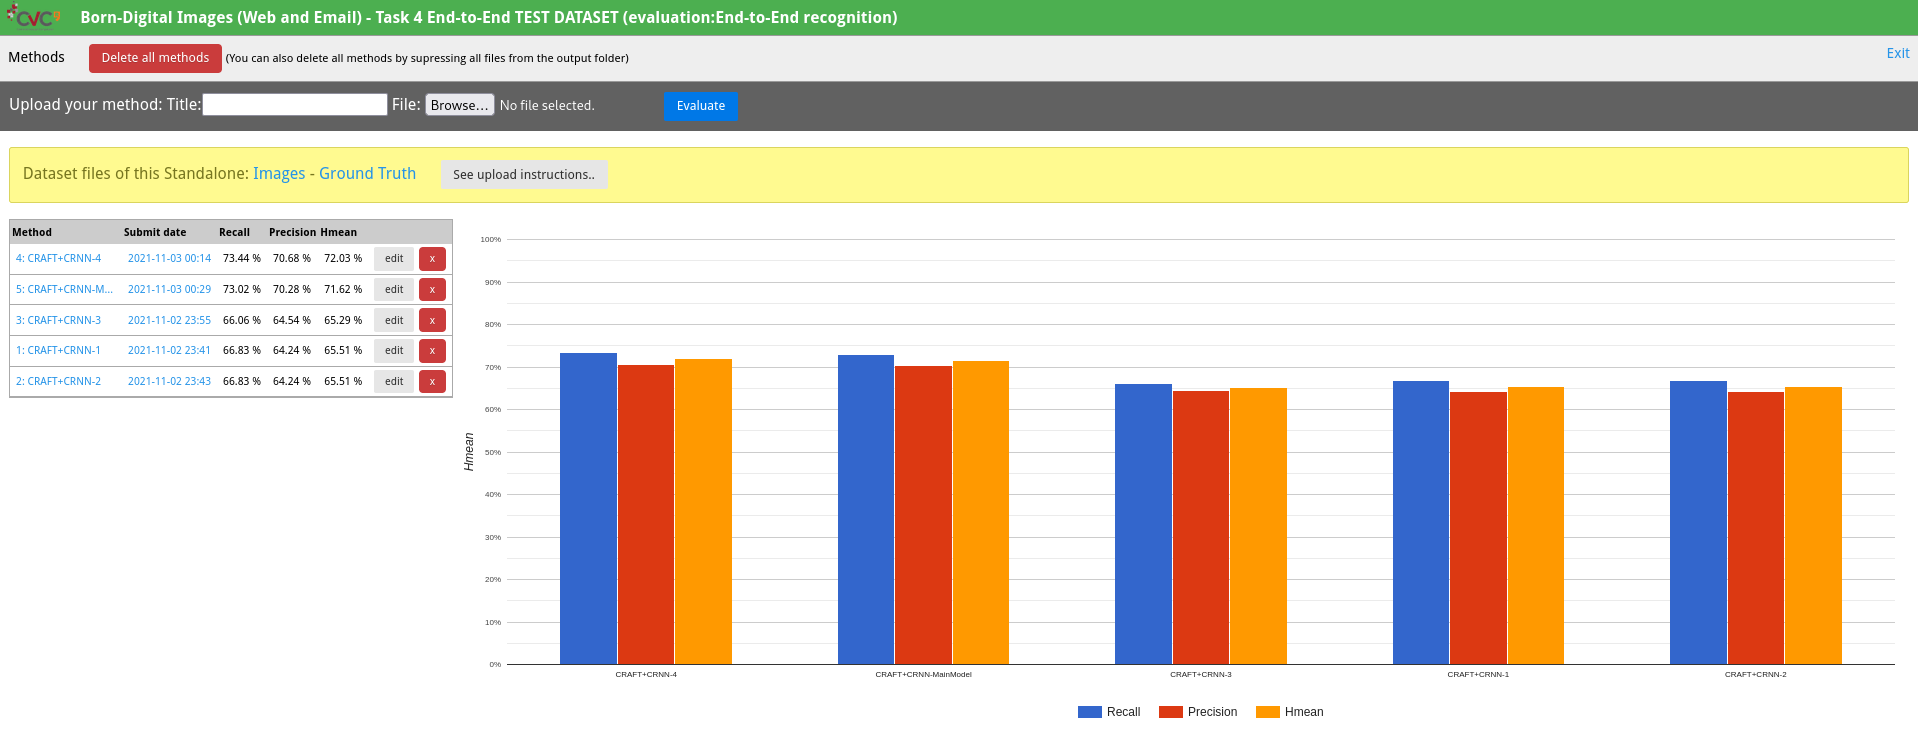
\includegraphics[width=0.8\textwidth]{figs/metodologia-interface-validacao.png}
    \caption{Interface de validação disponibilizada pela plataforma de desafios \textit{Robust Reading Competition}.}
    \label{fig:methodology_validation_interface}
\end{figure}

\begin{figure}
    \centering
    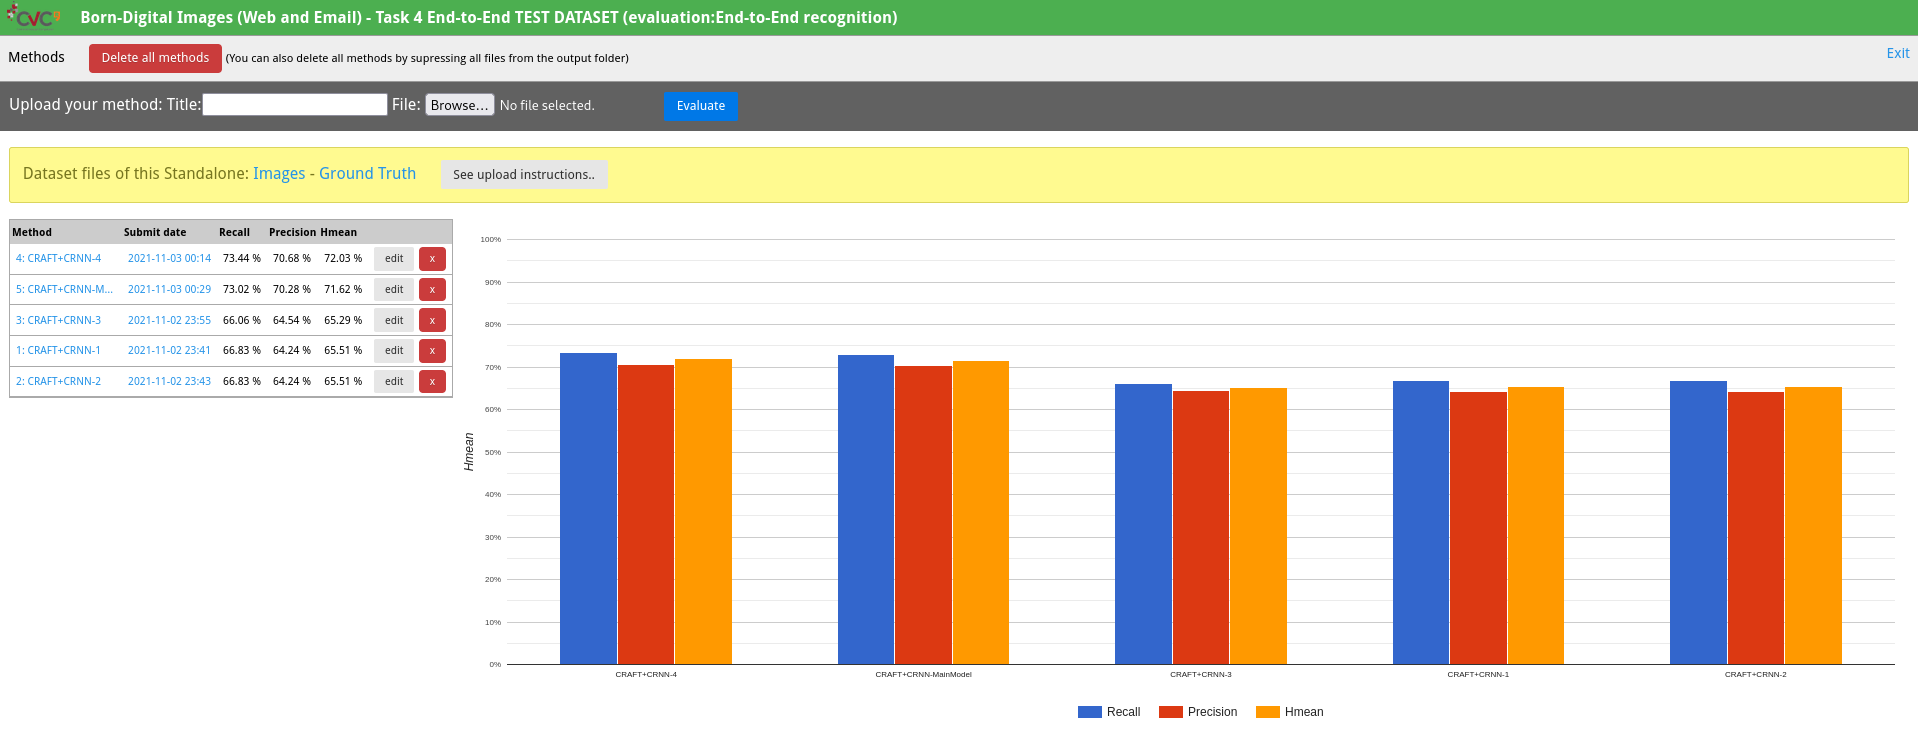
\includegraphics[width=0.8\textwidth]{figs/metodologia-interface-validacao.png}
    \caption{Interface de validação disponibilizada pela plataforma de desafios \textit{Robust Reading Competition}, com visualização de detalhes 
    da avaliação por imagem.}
    \label{fig:methodology_validation_interface_details}
\end{figure}

\section{Disponibilização da solução fim-a-fim em nuvem}\label{sec:methodology_cloud_deploy}
Uma vez com o desenvolvimento da integração entre os componentes concluída e avaliada, a próxima etapa para atingir os objetivos deste trabalho 
de graduação é executar uma prova de conceito sobre a solução proposta e disponibilizá-la em como uma aplicação \textit{web}, hospedada em nuvem, 
assim possibilitando demonstrar que seria possível distribuir a funcionalidade para outros consumidores, possivelmente evoluindo para um serviço 
digital de reconhecimento de texto, vendido como produto.

Existem diversas provedoras de computação em nuvem que poderiam ser utilizadas, entre as mais notáveis estão a gigante AWS\footnote{https://aws.amazon.com/pt} 
(Amazon Web Services) e a Paperspace, utilizada sob-demanda por esse trabalho durante o desenvolvimento conforme citado na Seção 
\ref{sec:metodologia_experimentacao}. Ambos serviços teriam infraestrutura para comportar a solução proposta por este trabalho, inclusive provendo 
máquinas com alto poder computacional dependendo da necessidade e dos limites financeiros do projeto. No entanto, apesar de ambos serviços possuírem 
limites de uso onde os recursos são gratuitos, não são de domínio do autor deste trabalho de graduação. Como uma terceira opção, a plataforma 
escolhida para hospedar o desenvolvimento deste trabalho foi o Heroku\footnote{https://heroku.com}. Apesar da escolha de uma plataforma específica 
para hospedar a aplicação, as ferramentas e o processo até a publicação em geral são comuns entre plataformas, então, resguardadas as devidas proporções, 
o processo feito para publicar a aplicação no Heroku pode ser extrapolado para algo similar em outros provedores de infraestrutura.

O Heroku uma plataforma disponibilizada pela empresa Salesforce\footnote{https://www.salesforce.com/} que age como uma camada de abstração sobre os 
provedores de nuvem e seus componentes de mais baixo nível, justamente para prover uma interface mais simples, facilitando a gestão de infraestrutura 
para desenvolvedores. As etapas para publicar uma aplicação para o Heroku envolvem poucos comandos e também pode hospedar aplicações usando recursos 
gratuitos. As limitações do ambiente gratuito e suas implicações na execução da aplicação serão abordadas no Capítulo \ref{cap:resultados}.

\subsection{Criação da Aplicação Web}\label{sec:methodology_web_app}
Até então, tudo que foi desenvolvido para este trabalho foi executado interagindo diretamente com os componentes da base de código, executando os 
\textit{scripts} de detecção e reconhecimento através de uma linha de comando pelo ambiente de desenvolvimento. Para expor o modelo integrado na Internet, 
desenvolveu-se uma aplicação \textit{web}, nos moldes de cliente-servidor, que responde requisições pelo protocolo HTTP, utilizando a arquitetura REST 
(\textit{Representational State Transfer}) de comunicação. Para isso foi necessário fazer algumas adições na base de código para contemplar a 
implementação de uma aplicação \textit{web} utilizando o framework Flask\footnote{https://flask.palletsprojects.com/en/2.1.x/}, que permite, com 
pouquíssima configuração, executar um servidor HTTP e possibilita que uma requisição seja atendida por um método da base de código.

Como o código existente esperava ser executado através dos \textit{scripts} diretamente, dependendo de parâmetros de linha de comando, foi necessário a 
criação de um novo arquivo contendo uma classe Python que centralizasse a execução dos métodos necessários para o funcionamento do reconhecimento 
fim-a-fim. Essa classe foi denominada \texttt{OcrRunner} e centraliza toda a orquestração do processamento, desde a preparação dos modelos junto ao 
framework PyTorch, até a execução de fato da detecção e do reconhecimento integradamente. Com isso, foi possível executar a solução fim-a-fim programaticamente.

Além da nova classe implementada, foi necessário desenvolver um método com a responsabilidade atender a requisição originada pelo cliente. Esse método, 
com a ajuda do framework Flask, consegue receber um arquivo de imagem enviado pelo cliente e executar a solução proposta sobre a imagem enviada. 
Por fim, quando o reconhecimento termina, o retorno do método é a lista de palavras reconhecidas, que, automaticamente, é respondido ao cliente que 
realizou a requisição.

Com essas poucas mudanças já é possível, de maneira miníma e muito simplificada, atender pedidos de reconhecimento de texto sob demanda. O próximo 
passo adotado utilizou ferramentas e conceitos voltados a conteinerização da aplicação para facilitar a execução no ambiente remoto, discutidos na 
próxima seção.

\subsection{Contêiner, Docker e Publicação}
Uma prática muito usual ao utilizar a computação em nuvem como meio de hospedar aplicações é gerar arquivos executáveis contendo tudo o que a aplicação 
precisa para funcionar: A base de código, as dependências, os binários, as configurações e tudo mais que for necessário, de maneira consistente e de 
fácil reprodutibilidade. Esse processo é por vezes chamado conteinerização, onde um contêiner é esse agregado do código da aplicação e tudo o que for 
ecessário para executá-la, de fato sendo executado. Uma das tecnologias de contêiner mais utilizadas é o Docker [\citeonline{Docker}]. Mais detalhes 
sobre Docker e contêineres podem ser encontrados na página oficial da tecnologia.

De modo a gerar um contêiner da aplicação desenvolvida neste trabalho, a primeiro etapa é descrever como esse contêiner é construído, e, para isso, 
cria-se um arquivo chamado \textit{Dockerfile}. No arquivo \textit{Dockerfile} deve constar uma série de comandos executados rigorosamente pelo Docker 
para criar uma imagem Docker. Ao executar a imagem pelo Docker, um novo processo, um contêiner, é inicializado com o conteúdo da imagem executada e 
pode executar o código compilado na imagem Docker. O arquivo Dockerfile pode ser consultado diretamente no repositório desse trabalho ou no 
Apêndice \ref{apd:dockerfile}.

Ter a aplicação “conteinerizada” economiza muita configuração na hora de publicá-la na nuvem, já que não se faz mais necessário configurar o servidor 
onde a aplicação será servida de forma específica para satisfazer as demandas de binários e bibliotecas para a aplicação em questão. Tudo o que é 
necessário para executar a aplicação já está definido na imagem do contêiner e estará pronto para uso quando o contêiner foi iniciado, dessa forma, 
as etapas mencionadas nas Seções \ref{sec:metodologia_experimentacao} e \ref{sec:metodologia_desenvolvimento} referentes a configuração do ambiente 
Python e instalação de dependências através do Conda já foi resolvido na criação da imagem e o ambiente já estará pronto para uso dentro do contêiner. 
O servidor que hospeda os contêineres não precisa saber de especificidades de cada aplicação, sua responsabilidade é saber executar os contêineres e 
compartilhar recursos computacionais com eles. Dessa forma, a publicação da aplicação no Heroku se resume a execução de um comando a interface de linha 
de comando que a plataforma disponibiliza para publicar uma aplicação a partir de uma imagem Docker.

\section{Considerações finais}
Sucintamente, nesse capítulo foi apresentado como ocorreu o desenvolvimento deste trabalho de graduação, mencionando como os modelos de detecção e 
reconhecimento foram escolhidos, como e com quais ferramentas eles foram testados, integrados e, ao final da integração como a solução foi validada 
e publicada em nuvem.

O próximo capítulo abordará mais a fundo os resultados do desenvolvimento, com enfoque na capacidade de detecção e reconhecimento do modelo integrado 
e discutindo um pouco sobre a execução da aplicação em nuvem.

\chapter{Resultados e Discussão}\label{cap:resultados}

\section{Detecção e Reconhecimento}
\subsection{ICDAR 2011}\label{sec:results_icdar_2011}
O conjunto de imagens de validação do ICDAR 2011 conta com 141 imagens e é importante de constatar que são imagens de relativa baixa resolução para os padrões atuais, onde as maiores contêm cerca de 315 mil pixels. São caracterizadas por estarem no contexto de imagens de anúncios e anexos de e-mails, com textos primariamente horizontais.

Ao aplicar a solução sobre os exemplos de validação do dataset, em termos de desempenho, todas as imagens foram processadas com sucesso em 36.31 segundos em um ambiente com aceleração gráfica, média de 257 ms por imagem. Para fins comparativos, a mesma tarefa agora executada sem a aceleração gráfica levou 328.44 segundos, cerca de 9 vezes mais tempo, executando na mesma máquina alocada no serviço Paperspace, que consta com 30GB de memória RAM, disponibilidade de processamento gráfico com NVIDIA QUADRO M4000 e processamento CPU baseado em instâncias AWS C4, disponibilizam 8 núcleos, 16 threads do processador Intel Xeon E5-2666, com clock de 2.9 GHz.

Apesar do maior tempo de processamento, o uso da solução em ambientes sem uma placa gráfica compatível ainda não se torna inviável, sobretudo considerando que a média de tempo de processamento por imagem foi de 2.32 segundos. No entanto, fica desencorajado a execução sobre um conjunto muito grande de imagens, já que o processamento corresponde a uma carga muito alta dependendo do hardware onde a solução for executada, uma vez que a execução em CPU alocou aproximadamente 17.4GB de memória, volume maior do que a quantidade total de grande parte dos sistemas mais domésticos.

Para executar o script de avaliação dos resultados da solução, o comando abaixo pode ser executado, fornecendo o caminho para um arquivo .ZIP que contém os arquivos de resultados para cada imagem do conjunto de validação.

\begin{minted}{bash}
            python script.py –g=gt.zip –s=res_img_.zip
\end{minted}

O resultado da melhor configuração foi o apresentado na Tabela \ref{tab:icdar11_results}. Em suma, a avaliação usa três métricas: Precisão, Recall e F1-Score. A Precisão é a relação dos acertos (verdadeiros positivos) sobre a contagem total de predições positivas (verdadeiros positivos e falsos positivos), ou seja, dentre as predições da solução, qual é a porcentagem de acerto. O Recall relaciona a quantidade de acertos com a quantidade total de casos verdadeiros. O F1-Score é basicamente a média harmônica das métricas Precisão e Recall.

\begin{minted}{bash}
                Calculated!
                {
                    "precision": 0.7068273092369478,
                    "recall": 0.7343532684283728,
                    "hmean": 0.7203274215552524, 
                    "AP": 0
                }
\end{minted}

\begin{table}[htb]
    \centering
    \caption{Avaliação de resultados sobre a base ICDAR 2011.}
    \begin{tabular}{|c|c|c|}
        \hline
        Precisão (\%) & Recall (\%) & F1-Score (\%) \\
        \hline
        70.68 & 73.44 & 72.03\\
        \hline
    \end{tabular}
    \label{tab:icdar11_results}
\end{table}

Em resumo, isso demonstra que a cada 100 palavras detectadas e processadas, aproximadamente 71 tiveram o texto corretamente extraído. É um resultado bem satisfatório para o trabalho desenvolvido e o nível de simplicidade que foi adotado. Estes números colocariam essa solução em nono lugar entre 18 outros trabalhos submetidos na plataforma de desafios Robust Reading Competition.

\begin{figure}
    \centering
    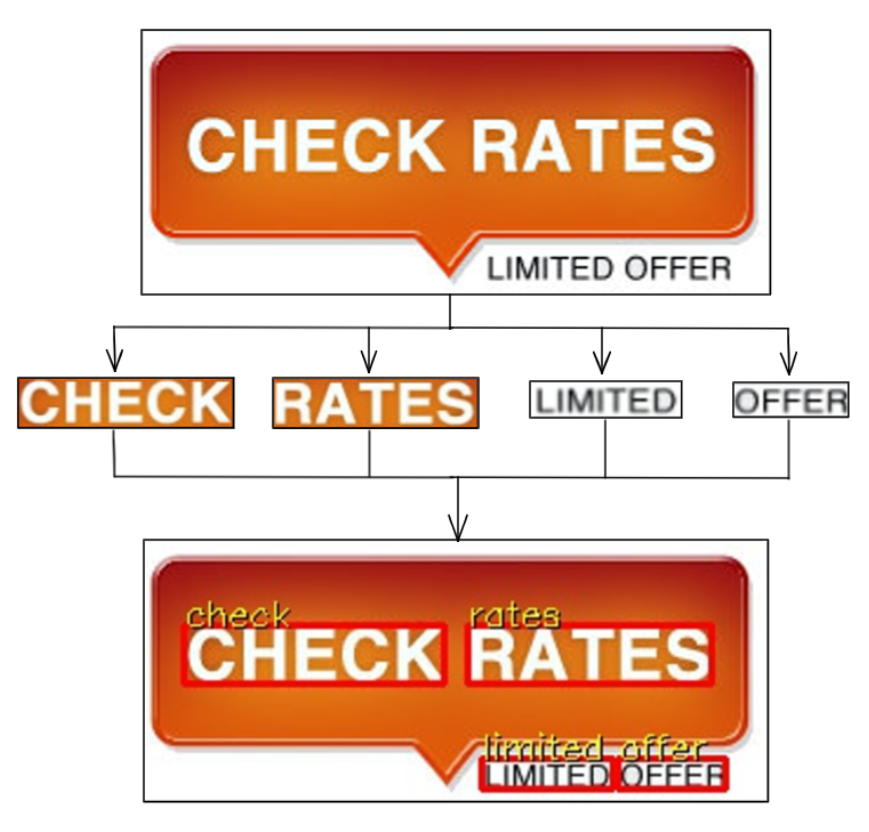
\includegraphics[width=0.5\textwidth]{figs/resultados-icdar11-01.png}
    \caption{Exemplo de resultado de reconhecimento. Imagem 52 do conjunto de validação.}
    \label{fig:results_icdar11_01}
\end{figure}

A Figura \ref{fig:results_icdar11_01} exemplifica as etapas da solução apresentada. A imagem de entrada é processada pela rede de detecção que extrai as regiões de texto regredindo as coordenadas das bounding-boxes. Com isso, essas regiões são então cortadas da imagem original e alimentam a rede de reconhecimento para extração do texto decodificado.

Apesar do resultado satisfatório, o mais interessante é aprofundar não nos acertos, onde o modelo reconheceu as palavras certas, mas sim onde ele errou e identificar limitações e, eventualmente, futuras otimizações.

Um dos casos mais evidentes onde a solução apresentou problemas foi na presença de caracteres especiais. Uma das limitações do modelo de reconhecimento é a lista de caracteres passíveis de reconhecimento, que contempla apenas os caracteres do alfabeto da língua inglesa, de A até Z, adicionado dos dígitos decimais, de 0 até 9. Este dicionário limitado restringe muito a capacidade de detecção em que não são tão difíceis de observar. Caracteres de pontuação, acentos, marcações como o cifrão (\$), entre outros casos, acabam dificultando o acerto do reconhecimento. A Figura \ref{fig:results_icdar11_02} exemplifica esta constatação. Nela, é possível observar que o trecho que representa o preço do item anunciado na imagem 5 do conjunto de validação, que contém cifrão, vírgula e asterisco, não foi reconhecida com sucesso. Apesar de o método aproximar bem os caracteres desconhecidos, reconhecendo o cifrão (\$) como um cinco (5) e o asterisco (*) como a letra X, o resultado não é satisfatório nesse caso.

\begin{figure}
    \centering
    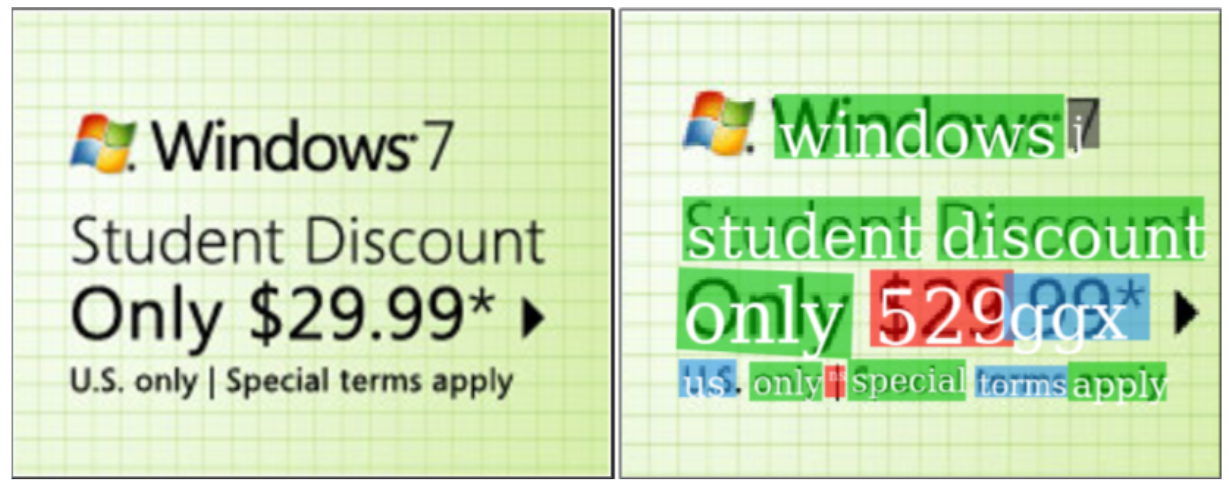
\includegraphics[width=0.75\textwidth]{figs/resultados-icdar11-02.png}
    \caption{Comparação entre entrada e saída sobre a imagem 5 do set de validação do ICDAR 2011}
    \label{fig:results_icdar11_02}
\end{figure}

Outra dificuldade ficou aparente em imagens de baixa resolução, que acabam contendo regiões de texto ainda menores. Em geral, a regressão das \textit{bounding-boxes} fica um pouco mais grosseira, mas ainda satisfatórias. Entretanto, a maior limitação foi o reconhecimento. As regiões de texto recortadas da imagem original acabam ficando bem pequenas e com pouca definição, o que trouxe dificuldades para o modelo pré-treinado CRNN utilizado. A Figura \ref{fig:results_icdar11_03} exemplifica essa dificuldade. Pode-se observar que nenhum dos "títulos" de cada uma das fotos que estão presentes na Figura \ref{fig:results_icdar11_03} foram localizadas com sucesso, mas não obtiveram a igualdade entre predição e gabarito (ficaram marcadas com uma área azul).

\begin{figure}
    \centering
    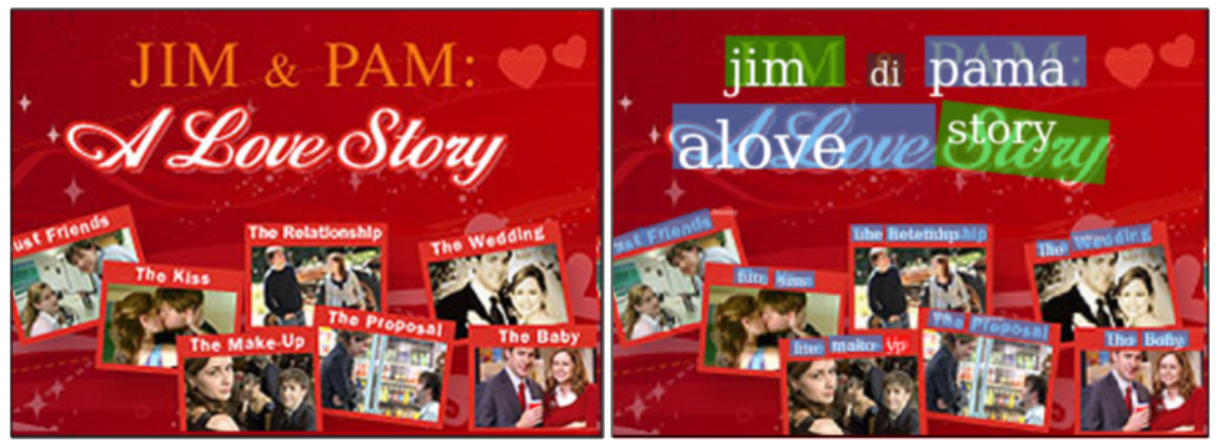
\includegraphics[width=0.75\textwidth]{figs/resultados-icdar11-03.png}
    \caption{Exemplo de imagem com instâncias de texto bem pequenas em resolução. Imagem 28 do ICDAR 2011}
    \label{fig:results_icdar11_03}
\end{figure}

Um outro detalhe que demonstra uma dificuldade mais global do problema de reconhecimento de texto em cenas é a fonte utilizada na frase “A Love Story”, na região superior da Figura \ref{fig:results_icdar11_03}. Apesar do reconhecimento ter relativo sucesso nesse exemplo, a localização não conseguiu segmentar corretamente todas as palavras da frase. A generalização da detecção e do reconhecimento para os mais diversos tipos de fontes é um dos principais problemas que motivam o uso de redes neurais profundas para reconhecimento de texto. [\citeonline{StrDlEra}]

O ICDAR 2011 apresenta casos mais complexos de detecção de reconhecimento de texto se comparado ao contexto de aplicações OCR convencionais, que lidam com reconhecimento de texto estruturado, sem grandes variações de fontes e planos de fundo, o que é bastante válido para avaliar a solução. No entanto, ainda não são casos reais de texto em cena, problema que motivou este trabalho. O dataset ICDAR 2013 contém exemplos mais característicos de texto de cena.

%%%%%%%%%%%%%%%%%%%%%%%%%%%%%%%%%%%%%%%%%%%%%%%%%%%%%%%%%%%%%%%%%%%%%%%%%%%%%%%%%%%%%%%%%%%%%%%%%%%%%%%%%%%%%%%%%%%%%%%%%%%%%%%%%%%%%%%%%%%%%%%%%%%%%%%%%%%%%%%%%%

\section{ICDAR 2013}\label{sec:results_icdar_2013}

O conjunto de imagens de validação do ICDAR 2013 conta com 233 imagens de tamanhos variados. As menores têm cerca de 640 pixels de altura e 480 pixels de comprimento, enquanto as maiores têm dimensões comparáveis à resolução 4K, com 3888 pixels de altura e 2592 pixels de comprimento. Vale ressaltar que as imagens passam por uma redução em resolução ao entrarem no modelo CRAFT, que maximiza a maior dimensão da imagem para 1280 pixels e ajusta a segunda dimensão mantendo a relação de aspecto original, justamente para otimizar o desempenho do método.

Ao aplicar a solução sobre os exemplos de validação do dataset, em termos de desempenho, todas as imagens foram processadas com sucesso em 207.74 segundos em um ambiente com aceleração gráfica, exatamente os mesmos recursos computacionais disponíveis na validação do ICDAR 2011, atingindo uma média de 892 ms por imagem. A média de tempo de processamento por imagem é cerca de 3.5 vezes maior quando comparado ao dataset anterior, ICDAR 2011.  As predições não foram executadas sem aceleração gráfica por economia de recursos.

Com base nas mesmas métricas apresentadas na Seção \ref{sec:results_icdar_2011}, durante a discussão sobre os resultados contra o ICDAR 2011, a avaliação da solução no ICDAR 2013 demonstra resultados similares aos vistos na Seção \ref{sec:results_icdar_2011}, disponíveis na Tabela \ref{tab:icdar13_results}. Cerca de 7 acertos a cada 10 predições. Tendo em vista que é uma base um pouco mais desafiadora, é um resultado novamente satisfatório. Comparando Precisão e Recall, nota-se um desvio maior, de aproximadamente 6 pontos percentuais, o que indica um maior número de falsos positivos, ou seja, regiões detectadas como regiões de texto que não estão nas anotações de gabarito. Em alguns casos, uma mesma palavra acabou sendo segmentada de maneira errada, em outros, regiões visivelmente de não-texto foram detectadas. A Figura \ref{fig:results_icdar13_01} demonstra esse fenômeno.


\begin{minted}{bash}
                Calculated!
                {
                    "precision": 0.7043390514631686,
                    "recall": 0.7611777535441657,
                    "hmean": 0.7316561844863733, 
                    "AP": 0
                }
\end{minted}

\begin{table}[htb]
    \centering
    \caption{Avaliação de resultados sobre a base ICDAR 2013.}
    \begin{tabular}{|c|c|c|}
        \hline
        Precisão (\%) & Recall (\%) & F1-Score (\%) \\
        \hline
        70.43 & 76.11 & 73.17\\
        \hline
    \end{tabular}
    \label{tab:icdar13_results}
\end{table}

\begin{figure}
    \centering
    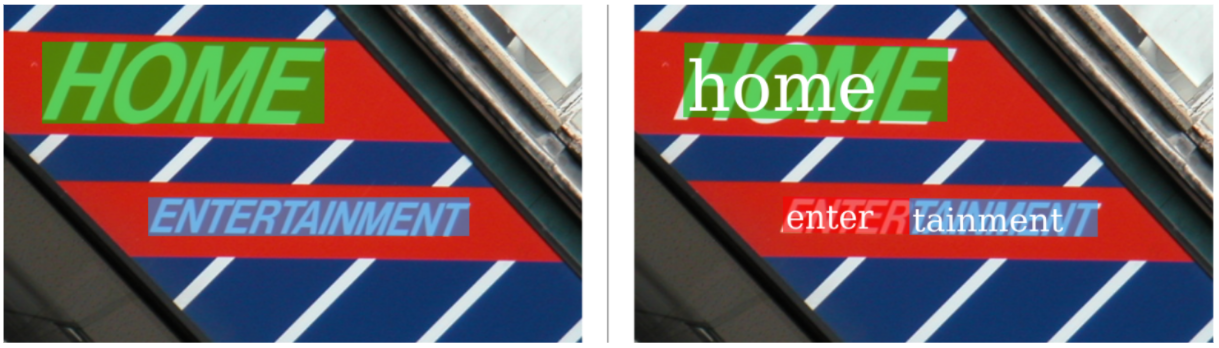
\includegraphics[width=0.75\textwidth]{figs/resultados-icdar13-01.png}
    \caption{Demonstração de um falso positivo durante a avaliação da solução contra o dataset ICDAR 2013}
    \label{fig:results_icdar13_01}
\end{figure}

Entretanto, as principais dificuldades de detecção e reconhecimento são compartilhadas com o que foi observado durante a avaliação na base ICDAR 2011. Caracteres especiais, pontuação e acentos são limitações conhecidas do reconhecimento.

Por introduzir mais exemplos de imagens verdadeiramente com textos em ambientes naturais, algumas novas dificuldades apareceram. O desafio que provavelmente é mais evidente está relacionado aos eventuais artefatos nas imagens decorrente de reflexos em algumas imagens de texto sob vidro ou com incidência de iluminação de alta intensidade (\textit{flashes} de câmeras fotográficas), onde, em alguns exemplos, a detecção foi sub-ótima (Figura \ref{fig:results_icdar13_03}) e em outros, o reconhecimento não foi o melhor (Figura \ref{fig:results_icdar13_02}).

\begin{figure}
    \centering
    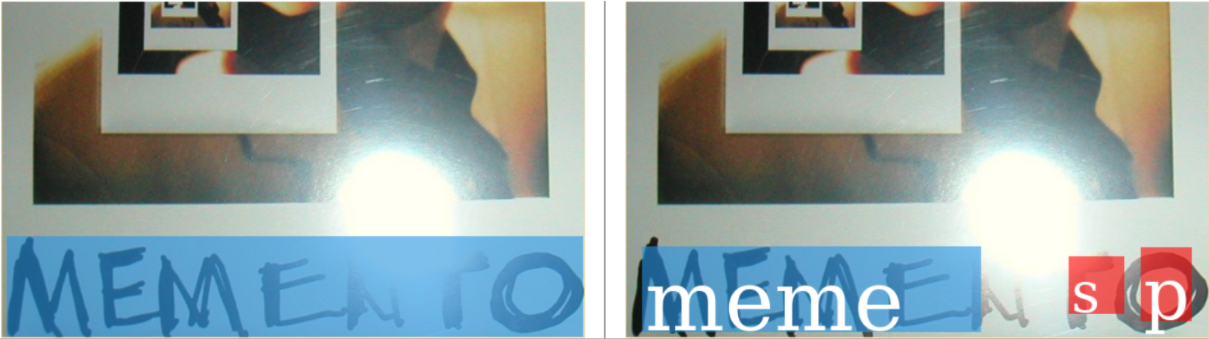
\includegraphics[width=0.75\textwidth]{figs/resultados-icdar13-03.png}
    \caption{Exemplo de imagem com artefatos que trouxeram dificuldades para a localização correta do texto.}
    \label{fig:results_icdar13_03}
\end{figure}

\begin{figure}
    \centering
    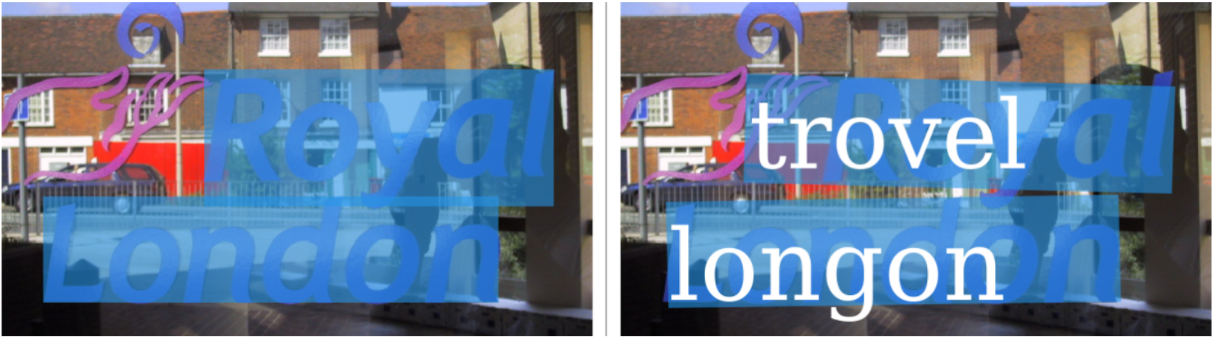
\includegraphics[width=0.75\textwidth]{figs/resultados-icdar13-02.png}
    \caption{Exemplo de texto sob vidro, com plano de fundo desafiadores para o reconhecimento.}
    \label{fig:results_icdar13_02}
\end{figure}

Outra dificuldade conhecida de problemas de reconhecimento de texto em cenas está relacionada a palavras em destaque, o que pode ser relativamente comum, dado o contexto de uma imagem com diversos objetos na cena. Apesar de ser um exemplo mais simples, a Figura \ref{fig:results_icdar13_04} demonstra esse caso. A etiqueta na infusão está visivelmente em desfoque e complicou o trabalho do reconhecimento por deixar os caracteres mais ambíguos.

\begin{figure}
    \centering
    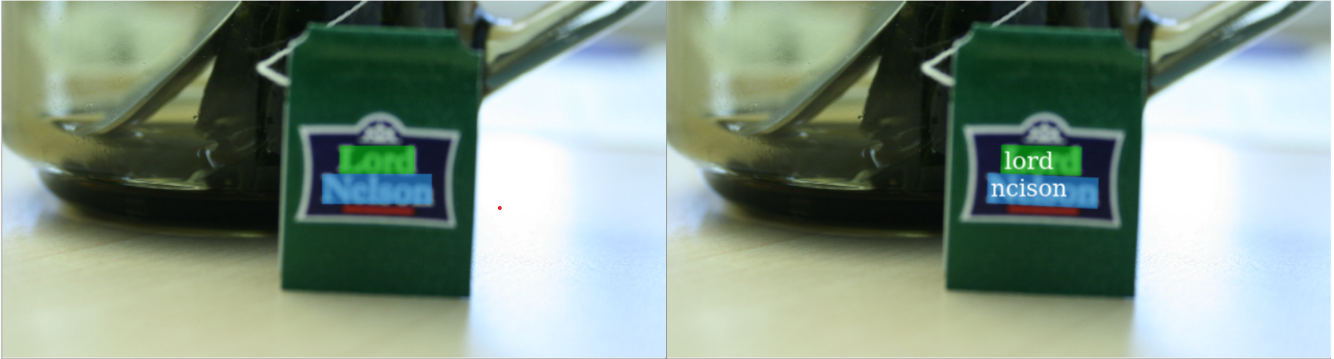
\includegraphics[width=\textwidth]{figs/resultados-icdar13-04.png}
    \caption{Exemplo de imagem com texto em desfoque}
    \label{fig:results_icdar13_04}
\end{figure}

%%%%%%%%%%%%%%%%%%%%%%%%%%%%%%%%%%%%%%%%%%%%%%%%%%%%%%%%%%%%%%%%%%%%%%%%%%%%%%%%%%%%%%%%%%%%%%%%%%%%%%%%%%%%%%%%%%%%%%%%%%%%%%%%%%%%%%%%

\subsection{Imagens autorais}\label{sec:results_own_images}
Com caráter mais qualitativo, é interessante inferir a qualidade das soluções em imagens fora do contexto de datasets conhecidamente utilizados para treino e validação, para experienciar a qualidade do reconhecimento em imagens do dia-a-dia. Com esse objetivo, algumas imagens no álbum pessoal do autor deste trabalho foram selecionadas para passarem pela solução apresentada. Alguns exemplos estão disponíveis abaixo.

\begin{figure}
    \centering
    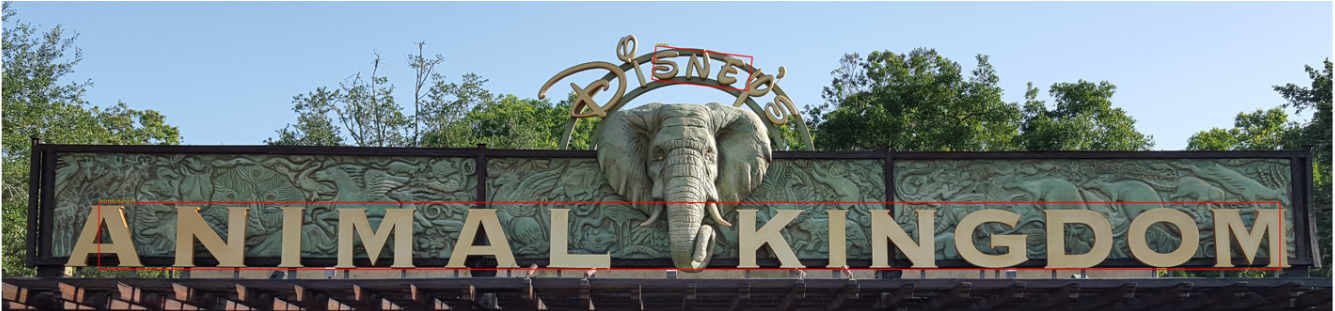
\includegraphics[width=\textwidth]{figs/resultados-autoral-01.png}
    \caption{Exemplo de imagem autoral onde a solução apresentou dificuldades com texto curvo e estilizado. Textos reconhecidos: “sney” e “intmalakingon”.}
    \label{fig:results_own_images_01}
\end{figure}

\begin{figure}
    \centering
    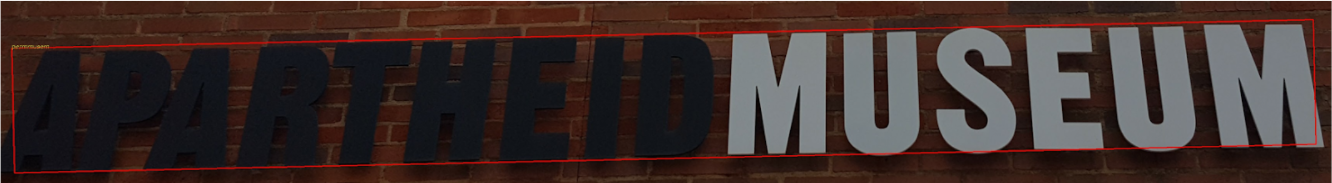
\includegraphics[width=\textwidth]{figs/resultados-autoral-02.png}
    \caption{Exemplo de imagem autoral onde uma região de texto muito longa não foi extraída muito bem, principalmente no início da palavra, o que dificultou o reconhecimento. Texto reconhecido: “permmusem”.}
    \label{fig:results_own_images_02}
\end{figure}

Algumas imagens utilizadas foram bastante desafiadoras para a solução, tanto em termos de localização quanto reconhecimento. Imagens com texto bem localizado e visível, alguns letreiros e placas tiveram bons resultados, mas alguns casos de palavras mais longas e curvadas, mesmo que levemente, não tiveram muito sucesso, especialmente se apresentarem caligrafia muito estilizadas, como é possível observar na Figura \ref{fig:results_own_images_03}. A respeito de textos curvados, melhorias na solução poderiam melhorar a situação, como a aplicação de soluções para transformar as imagens antes de passar pelo reconhecimento como, por exemplo, uma rede STN (\textit{Spatial Transformer Network} \cite{STN}), a fim de obter uma imagem com o mínimo de curvatura possível, facilitando o trabalho de reconhecimento.

\begin{figure}
    \centering
    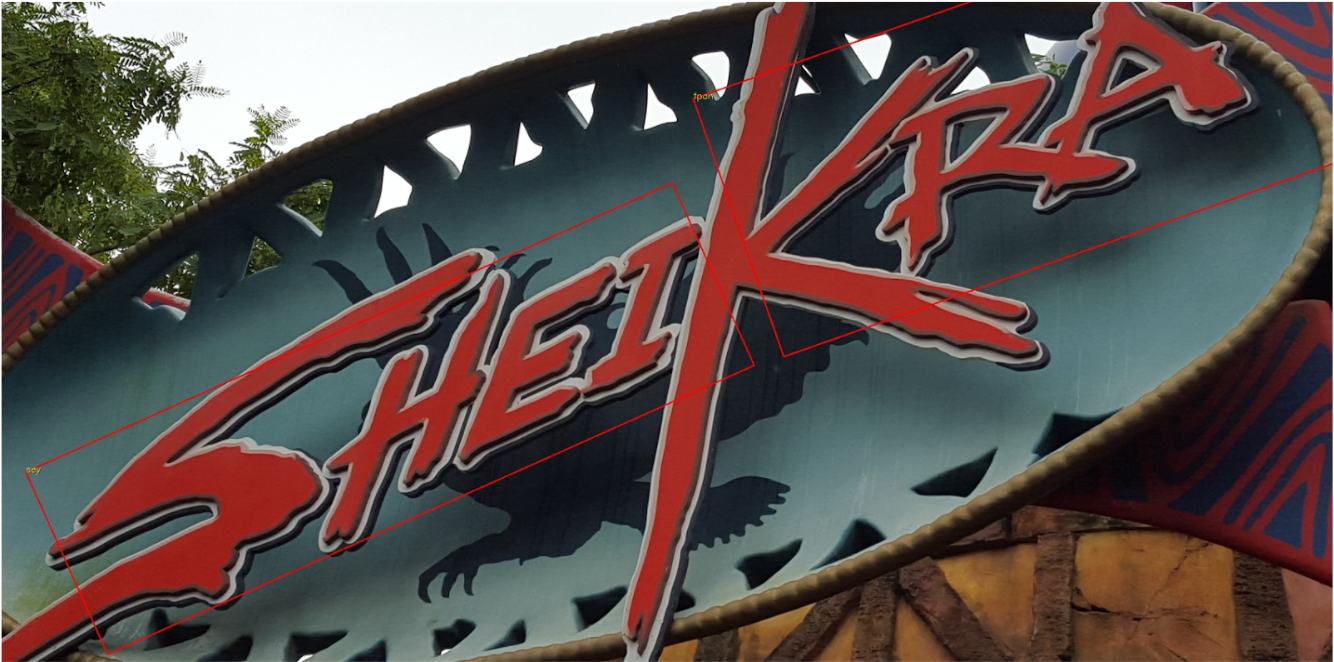
\includegraphics[width=0.7\textwidth]{figs/resultados-autoral-03.png}
    \caption{Exemplo de imagem autoral com fontes bastante estilizadas que trouxeram dificuldade tanto para a detecção, quanto para o reconhecimento. Textos reconhecidos: “sey” e “fpan”.}
    \label{fig:results_own_images_03}
\end{figure}


Um exemplo foi bastante interessante, pois contrariou as expectativas quanto ao reconhecimento, o que demonstra o potencial que a solução pode apresentar com algumas iterações de melhorias. A Figura \ref{fig:results_own_images_04} mostra um caso de sucesso na localização e reconhecimento onde o contexto no qual o texto está inserido tem bastante informação e a fonte do texto, principalmente do trecho escrito “Disney’s”, é bastante estilizado, e mesmo assim, o reconhecimento foi bem preciso.


Agora, quando o texto se encontra em situações bastante favoráveis, por exemplo, bem iluminado, sem oclusões, em geral disposto horizontalmente e com caligrafia não rebuscada, a solução atinge o seu potencial máximo, conseguindo localizar e interpretar com muita precisão. A Figura \ref{fig:results_own_images_05} demonstra esse caso, onde temos um cartaz de boas-vindas do museu do Apartheid, na Africa do Sul.

\begin{figure}
    \centering
    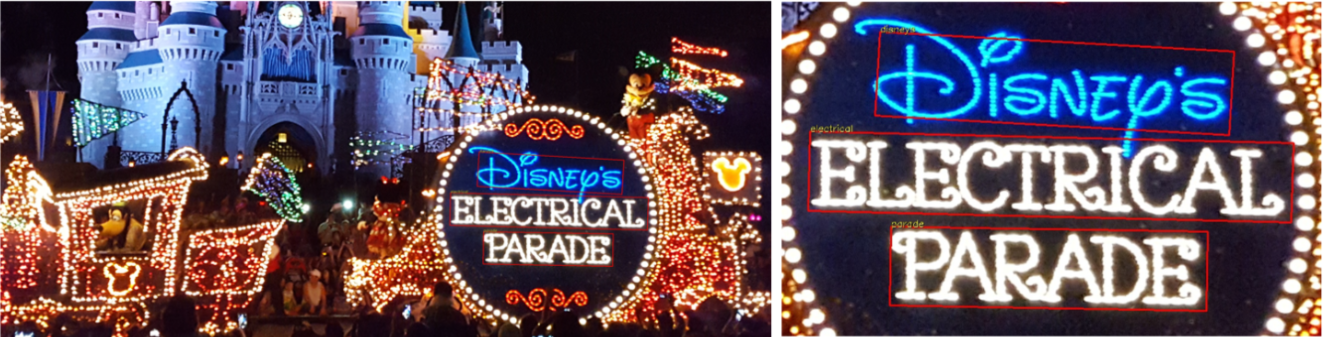
\includegraphics[width=\textwidth]{figs/resultados-autoral-04.png}
    \caption{Exemplo de reconhecimento com sucesso em condições desafiadoras em imagem autoral. Textos reconhecidos: “disneys”, "electrical" e “parade”.}
    \label{fig:results_own_images_04}
\end{figure}

\begin{figure}
    \centering
    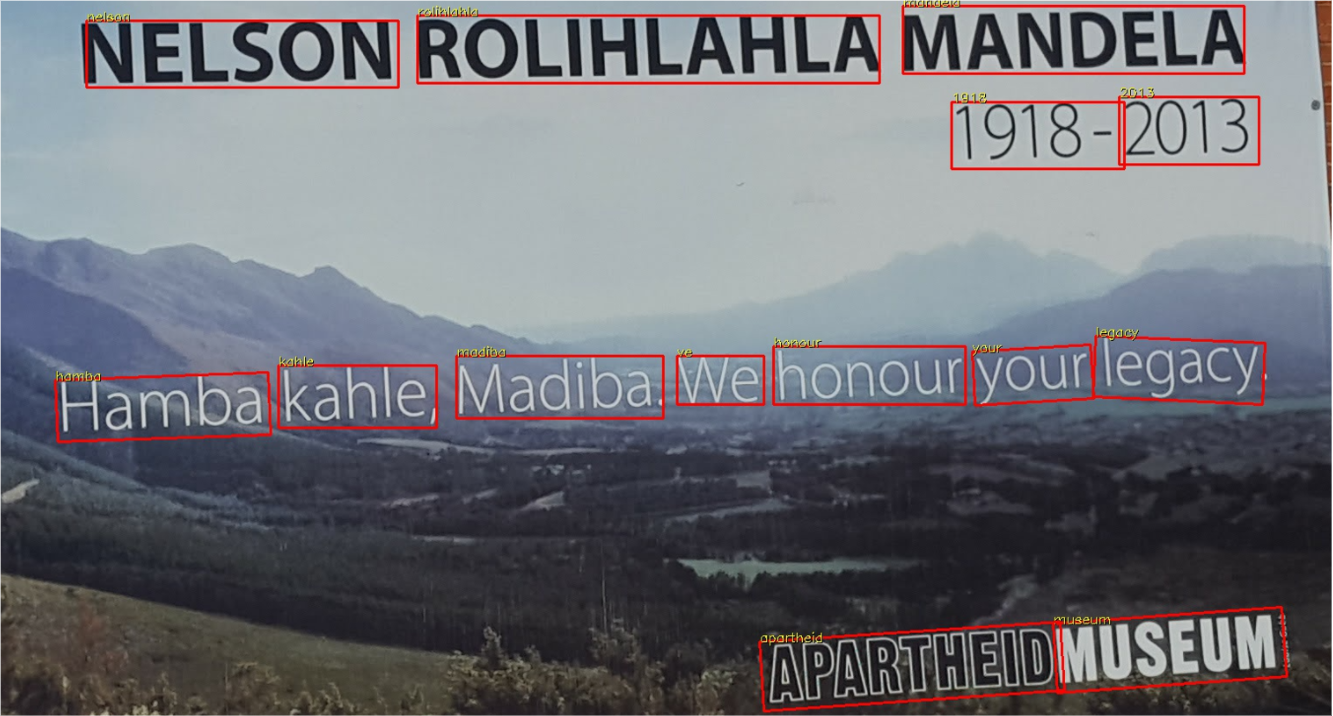
\includegraphics[width=0.75\textwidth]{figs/resultados-autoral-05.png}
    \caption{Exemplo de imagem autoral com alta precisão de reconhecimento. Textos reconhecidos: “nelson”, “rolihlahla” “mandela”, “1918”, “2013”, “hamba”, “kahle”, “madiba”, “ve”, “honour”, “your”, “legacy”, “apartheid”, “museum”.}
    \label{fig:results_own_images_05}
\end{figure}


\section{Disponibilização em nuvem}
O resultado final da prova de conceito de publicar a aplicação final em um ambiente remoto através de computação em nuvem foi de relativo sucesso. Ao final de todas as etapas citadas em \ref{sec:methodology_cloud_deploy}, a aplicação foi publicada na plataforma do Heroku com sucesso. No entanto, como constatado na Seção \ref{sec:results_icdar_2011}, a demanda de recursos computacionais da solução integrada foi é relativamente grande, em especial a pressão sobre disponibilidade de memória RAM no sistema é grande.

O ambiente que é disponibilizado de graça pelo Heroku é bastante limitado em recursos, por questões óbvias, portanto já não era esperado uma boa performance, sobretudo pelo fato do ambiente não contar com aceleração gráfica.

A partir de alguns testes sobre aplicação publicada, pode-se observar que o ambiente não é de fato estável para a aplicação que foi publicada. Ao requisitar a execução do reconhecimento em imagens menores do dataset ICDAR 2011, com dimensões próximas de 300px por 300px ainda é possível obter uma resposta do servidor, porém para imagens maiores e mais pesadas, a aplicação ultrapassa os limites de memória que tem disponível para o contêiner e, como medida de segurança imposta pelo Heroku, o contêiner é desligado sem conseguir terminar o processo de reconhecimento.
\chapter{Conclusão}

Ao fim de todo o desenvolvimento desse trabalho de graduação a fim de recapitulação, observa-se uma solução capaz 
de reconhecer textos em fotografias onde as palavras ou instâncias de texto não necessariamente foram a motivação 
da fotografia e, em geral, não são documentos com texto impresso ou manuscrito em papel. Essas imagens são características 
do problema de \textit{Scene Text Recognition} (STR).

A partir do re-uso de um detector e um reconhecedor de texto, populares em trabalhos na área, foi possível implementar 
e avaliar a integração dos dois métodos, obtendo no final uma composição capaz de resolver o problema de STR na 
maneira dita fim-a-fim, agregando as etapas de detecção e reconhecimento de uma vez só, com capacidade de acertar o 
reconhecimento em 70\% das vezes, o que não é o melhor resultado observado no meio acadêmico, mas considerando que 
simplificações foram feitas para possibilitar a implementação, é um resultado satisfatório e cumpre o objetivo do trabalho.

Como observado, a solução desenvolvida apresentou dificuldades nos exemplos de avaliação e no ambiente remoto 
provisionado na nuvem e possibilidades de evolução para trabalhos futuros podem tentar atacá-las, como, por exemplo, 
refinar os parâmetros do modelo de detecção para melhorar os resultados para textos mais longos e textos não-horizontais, 
implementar método de transformação da região de texto para melhorar resultados do reconhecimento, treinar um novo modelo de 
reconhecimento com um dicionário maior de caracteres e até tentar otimizar o uso de recursos computacionais da solução.


% ----------------------------------------------------------
% ELEMENTOS PÓS-TEXTUAIS (Referências, Glossário, Apêndices)
% ----------------------------------------------------------
\postextual

% Referências bibliográficas
\bibliography{bibliografia}

% Glossário (Consulte o manual)
%\glossary

% Apêndices
% ----------------------------------------------------------
% Apêndices
% ----------------------------------------------------------

% ---
% Inicia os apêndices
% ---
\begin{apendicesenv}

% Imprime uma página indicando o início dos apêndices
\partapendices

% ----------------------------------------------------------
\chapter{Arquivo de descrição do ambiente virtual Conda utilizado no desenvolvimento}\label{apd:yaml-desenvolvimento}
% ---
\begin{minted}{yaml}
name: craft-detector
channels:
  - defaults
dependencies:
  - _libgcc_mutex=0.1=main
  - _openmp_mutex=4.5=1_gnu
  - _pytorch_select=0.1=cpu_0
  - blas=1.0=mkl
  - bzip2=1.0.8=h7b6447c_0
  - ca-certificates=2021.10.26=h06a4308_2
  - cairo=1.16.0=hf32fb01_1
  - certifi=2021.10.8=py37h06a4308_2
  - cffi=1.14.6=py37h400218f_0
  - click=8.0.3=pyhd3eb1b0_0
  - cloudpickle=2.0.0=pyhd3eb1b0_0
  - cycler=0.10.0=py37_0
  - cytoolz=0.11.0=py37h7b6447c_0
  - dask-core=2021.8.1=pyhd3eb1b0_0
  - dataclasses=0.8=pyh6d0b6a4_7
  - dbus=1.13.18=hb2f20db_0
  - expat=2.4.1=h2531618_2
  - ffmpeg=4.0=hcdf2ecd_0
  - flask=2.0.2=pyhd3eb1b0_0
  - fontconfig=2.13.1=h6c09931_0
  - freeglut=3.0.0=hf484d3e_5
  - freetype=2.10.4=h5ab3b9f_0
  - fsspec=2021.8.1=pyhd3eb1b0_0
  - glib=2.69.1=h5202010_0
  - graphite2=1.3.14=h23475e2_0
  - gst-plugins-base=1.14.0=h8213a91_2
  - gstreamer=1.14.0=h28cd5cc_2
  - harfbuzz=1.8.8=hffaf4a1_0
  - hdf5=1.10.2=hba1933b_1
  - icu=58.2=he6710b0_3
  - imageio=2.9.0=pyhd3eb1b0_0
  - intel-openmp=2019.4=243
  - itsdangerous=2.0.1=pyhd3eb1b0_0
  - jasper=2.0.14=h07fcdf6_1
  - jinja2=3.0.2=pyhd3eb1b0_0
  - jpeg=9d=h7f8727e_0
  - kiwisolver=1.3.1=py37h2531618_0
  - lcms2=2.12=h3be6417_0
  - ld_impl_linux-64=2.35.1=h7274673_9
  - libffi=3.3=he6710b0_2
  - libgcc-ng=9.3.0=h5101ec6_17
  - libgfortran-ng=7.5.0=ha8ba4b0_17
  - libgfortran4=7.5.0=ha8ba4b0_17
  - libglu=9.0.0=hf484d3e_1
  - libgomp=9.3.0=h5101ec6_17
  - libmklml=2019.0.5=0
  - libopencv=3.4.2=hb342d67_1
  - libopus=1.3.1=h7b6447c_0
  - libpng=1.6.37=hbc83047_0
  - libstdcxx-ng=9.3.0=hd4cf53a_17
  - libtiff=4.2.0=h85742a9_0
  - libuuid=1.0.3=h1bed415_2
  - libvpx=1.7.0=h439df22_0
  - libwebp-base=1.2.0=h27cfd23_0
  - libxcb=1.14=h7b6447c_0
  - libxml2=2.9.12=h03d6c58_0
  - locket=0.2.1=py37h06a4308_1
  - lz4-c=1.9.3=h295c915_1
  - markupsafe=2.0.1=py37h27cfd23_0
  - matplotlib=3.3.2=h06a4308_0
  - matplotlib-base=3.3.2=py37h817c723_0
  - mkl=2020.2=256
  - mkl-service=2.3.0=py37he8ac12f_0
  - mkl_fft=1.3.0=py37h54f3939_0
  - mkl_random=1.1.1=py37h0573a6f_0
  - ncurses=6.2=he6710b0_1
  - networkx=2.6.2=pyhd3eb1b0_0
  - ninja=1.10.2=hff7bd54_1
  - numpy=1.19.2=py37h54aff64_0
  - numpy-base=1.19.2=py37hfa32c7d_0
  - olefile=0.46=py37_0
  - opencv=3.4.2=py37h6fd60c2_1
  - openjpeg=2.4.0=h3ad879b_0
  - openssl=1.1.1m=h7f8727e_0
  - packaging=21.0=pyhd3eb1b0_0
  - partd=1.2.0=pyhd3eb1b0_0
  - pcre=8.45=h295c915_0
  - pillow=8.3.1=py37h2c7a002_0
  - pip=21.2.2=py37h06a4308_0
  - pixman=0.40.0=h7f8727e_1
  - py-opencv=3.4.2=py37hb342d67_1
  - pycparser=2.20=py_2
  - pyparsing=2.4.7=pyhd3eb1b0_0
  - pyqt=5.9.2=py37h05f1152_2
  - python=3.7.11=h12debd9_0
  - python-dateutil=2.8.2=pyhd3eb1b0_0
  - pytorch=1.8.1=cpu_py37h60491be_0
  - pywavelets=1.1.1=py37h7b6447c_2
  - pyyaml=5.4.1=py37h27cfd23_1
  - qt=5.9.7=h5867ecd_1
  - readline=8.1=h27cfd23_0
  - scikit-image=0.14.2=py37he6710b0_0
  - scipy=1.1.0=py37h7c811a0_2
  - setuptools=58.0.4=py37h06a4308_0
  - sip=4.19.8=py37hf484d3e_0
  - six=1.16.0=pyhd3eb1b0_0
  - sqlite=3.36.0=hc218d9a_0
  - tbb=2021.3.0=hd09550d_0
  - tbb4py=2021.3.0=py37hd09550d_0
  - tk=8.6.11=h1ccaba5_0
  - toolz=0.11.1=pyhd3eb1b0_0
  - torchvision=0.2.1=py37_0
  - tornado=6.1=py37h27cfd23_0
  - typing-extensions=3.10.0.2=hd3eb1b0_0
  - typing_extensions=3.10.0.2=pyh06a4308_0
  - werkzeug=2.0.2=pyhd3eb1b0_0
  - wheel=0.37.0=pyhd3eb1b0_1
  - xz=5.2.5=h7b6447c_0
  - yaml=0.2.5=h7b6447c_0
  - zlib=1.2.11=h7b6447c_3
  - zstd=1.4.9=haebb681_0
prefix: /var/home/mmilani/.conda/envs/craft-detector
\end{minted}
% ----------------------------------------------------------

% ----------------------------------------------------------
\chapter{Arquivo de descrição do ambiente virtual Conda utilizado durante a validação}\label{apd:yaml-validacao}
% ---
\begin{minted}{yaml}
name: str-eval
channels:
  - defaults
dependencies:
  - _libgcc_mutex=0.1=main
  - _openmp_mutex=4.5=1_gnu
  - ca-certificates=2021.10.26=h06a4308_2
  - certifi=2021.10.8=py37h06a4308_0
  - ld_impl_linux-64=2.35.1=h7274673_9
  - libffi=3.3=he6710b0_2
  - libgcc-ng=9.3.0=h5101ec6_17
  - libgomp=9.3.0=h5101ec6_17
  - libstdcxx-ng=9.3.0=hd4cf53a_17
  - ncurses=6.2=he6710b0_1
  - openssl=1.1.1l=h7f8727e_0
  - pip=21.0.1=py37h06a4308_0
  - python=3.7.11=h12debd9_0
  - readline=8.1=h27cfd23_0
  - setuptools=58.0.4=py37h06a4308_0
  - sqlite=3.36.0=hc218d9a_0
  - tk=8.6.11=h1ccaba5_0
  - wheel=0.37.0=pyhd3eb1b0_1
  - xz=5.2.5=h7b6447c_0
  - zlib=1.2.11=h7b6447c_3
  - pip:
    - numpy==1.21.3
    - polygon3==3.0.9.1
prefix: /var/home/mmilani/.conda/envs/str-eval
\end{minted}
% ----------------------------------------------------------

% ----------------------------------------------------------
\chapter{Arquivo Dockerfile utilizado na implantação da aplicação em nuvem}\label{apd:dockerfile}
% ---
\begin{minted}{dockerfile}
FROM continuumio/miniconda3:latest

ARG FLASK_ENV='production'
ENV FLASK_ENV $FLASK_ENV
ENV FLASK_APP '/app/app.py'

WORKDIR /app
COPY ./requirements-cpu.yml /app/requirements-cpu.yml
RUN conda env create -f /app/requirements-cpu.yml

ADD . /app

CMD [
    "conda",
    "run",
    "--no-capture-output",
    "-n",
    "craft-detector",
    "flask",
    "run",
    "--host=0.0.0.0",
    "--port=\$PORT"
]
\end{minted}
% ----------------------------------------------------------

\chapter{Exemplo de arquivo de resultado para avaliação}\label{apd:exe_resultado}
% ---
\begin{minted}{text}
3181,1200,3574,1200,3574,1278,3181,1278,mandela
2622,1211,3154,1211,3154,1289,2622,1289,rolihlahla
2241,1217,2600,1217,2600,1294,2241,1294,nelson
3430,1305,3591,1305,3591,1383,3430,1383,2013
3237,1311,3436,1311,3436,1388,3237,1388,1918
3403,1581,3598,1589,3595,1660,3400,1651,legacy
3032,1593,3253,1593,3253,1660,3032,1660,honour
3261,1599,3397,1591,3401,1653,3264,1661,your
2667,1604,2905,1604,2905,1676,2667,1676,madiba
2921,1604,3021,1604,3021,1660,2921,1660,ve
2462,1615,2644,1615,2644,1687,2462,1687,kahle
2205,1632,2450,1623,2453,1695,2208,1703,hamba
3354,1913,3617,1894,3623,1974,3359,1993,museum
3016,1934,3362,1911,3367,1990,3021,2014,apartheid
\end{minted}
% ----------------------------------------------------------


\end{apendicesenv}
% ---

% Anexos
%% ----------------------------------------------------------
% Apêndices
% ----------------------------------------------------------

% ---
% Inicia os anexos
% ---
\begin{anexosenv}

% Imprime uma página indicando o início dos anexos
\partanexos

% ---
\chapter{Nome do Primeiro Anexo}
% ---
\lipsum[30] % Texto qualquer. REMOVER!!

% ---
\chapter{Nome de Outro Anexo}
% ---

\lipsum[32] % Texto qualquer. REMOVER!!

\end{anexosenv}

% Índice remissivo (Consultar manual)
%\phantompart
%\printindex

\end{document}
